% !TeX root = RJwrapper.tex
\title{BCClong: An R Package for Bayesian Consensus Clustering for Multiple Longitudinal Features}
\author{ Zhiwen Tan,  Chang Shen, Zihang Lu}
\maketitle
\abstract{%
It is very common nowadays for a study to collect multiple longitudinal features, and appropriately integrating these features simultaneously for defining individual subgroups (i.e., clusters) becomes increasingly crucial to understanding population heterogeneity and predicting future outcomes. The aim of this paper is to describe a new package, BCClong, which implements a Bayesian consensus clustering (BCC) model for multiple longitudinal features. Compared to existing packages, several key features make the BCClong package appealing: (a) it allows simultaneous clustering of mixed-type (e.g., continuous, discrete, and categorical) longitudinal features, (b) it allows each longitudinal feature to be collected from different sources, with measurements taken at distinct sets of time points (known as irregularly sampled longitudinal data), and (c) it relaxes the assumption that all features have the same clustering structure by estimating the feature-specific (local) clusterings and consensus (global) clustering. Using two real data examples, we provide a tutorial with step-by-step instructions on how to use the package.
}
\section[Introduction]{Introduction} \label{sec:intro}
Cluster analysis has been widely used to identify subgroups of the study population, and it is also known as an unsupervised learning method in the machine learning literature. When longitudinal data is available, identifying distinct developmental patterns is a common goal in many research studies. Traditional statistical models often focus on clustering a single longitudinal feature, which may ignore the complexity of the clustering structures and the dynamic relationship when multiple longitudinal features are available. It is very common nowadays for a study to collect multiple features, and appropriately integrating multiple longitudinal features simultaneously for defining individual subgroups (i.e., clusters) becomes increasingly crucial to understanding population heterogeneity and predicting future outcomes. In particular, compared to clustering a single longitudinal feature, simultaneously clustering multiple longitudinal features (also known as joint clustering) facilitates the discovery of co-occurring trajectory patterns for multiple features of interest.
Several R packages have been developed to cluster longitudinal data with multiple features. For model-based clustering, the \pkg{gbmt} package \citep{Magrini2022} and the \pkg{flexmix} package \citep{Leisch2004} are developed to implement the group-based multi-trajectory analysis (GBMT) \citep{Nagin2018, Magrini2022a}. Both packages implement the EM algorithm, allowing unbalanced data and missing values, and can only be applied to continuous features. Notably, a SAS procedure PROC TRAJ is also developed for this model and has been widely used \citep{Nagin2018}. The GBMT assumes that the features and repeated measures are independent conditional on the cluster membership. Alternatively, the \pkg{lcmm} and \pkg{mixAK} packages are developed under the framework of mixed-effect models. The dependence between features and repeated measurements is captured by joint modeling of the random effects. Specifically, the \pkg{lcmm} package is designed for performing analyses such as latent class mixed models for a single longitudinal feature, joint latent class mixed models for multiple longitudinal features, as well as joint latent class mixed models for longitudinal features and time-to-event outcomes. While this package allows modeling multiple continuous or categorical longitudinal data of the same type, it does not support clustering mixed data types (e.g., continuous and categorical) simultaneously. On the other hand, the \pkg{mixAK} package can handle same-type (e.g., multiple continuous) or mixed-type (e.g., continuous, discrete, and categorical) features. For nonparametric clustering, the \pkg{kml3d} package \citep{Genolini2013} is developed to implement the K-means clustering for multiple longitudinal features, which is an extension of the \pkg{kml} package \citep{Genolini2010} for a single longitudinal feature. However, this package can only be applied to continuous features and does not allow for missing data. See \citet{Lu2023} for a review and comparison of these packages.
The aim of this paper is to describe a new package, the \pkg{BCClong} package, which implements the BCC model for multiple longitudinal features \citep{Lu2022,Tan2022a}. Compared to existing packages, several key features make the \pkg{BCClong} package appealing: (a) it allows simultaneous clustering of mixed-type (e.g., continuous, discrete, and categorical) longitudinal features, (b) it allows each longitudinal feature to be collected from different sources, with measurements taken at distinct sets of time points (known as irregularly sampled longitudinal data), and (c) it relaxes the assumption that all features have the same clustering structure by estimating the feature-specific (local) clusterings and overall (global) clustering. This model is very flexible, which facilitates the interpretation of clustering results and enhances its practical utilities. 
\section{Models and software} \label{sec:models}
The methodology of the BCC model for clustering multiple longitudinal features implemented in the \pkg{BCClong} package is described in detail in \citet{Lu2022} (for multiple continuous features) and in \citet{Tan2022a} (for multiple mixed-type features). In this section, we provide a brief overview of this model and the \pkg{BCClong} package. Without loss of generality, we use the term "features" to represent variables of interest used for the cluster analysis; however, these variables can also be a patient's traits, biomarkers, risk factors, exposures, and outcomes of interest in different contexts and studies.
\subsection{Bayesian Consensus Clustering for Multiple Longitudinal Features}
The BCC model is originally proposed as a flexible approach to model the dependence and heterogeneity of the data collected from multiple sources \citep{Lock2013}. Instead of arriving at a single overall clustering structure, the BCC model allows each feature to follow feature-specific (local) clustering and these local clusterings are aggregated to find a consensus (global) clustering.
Let $L_{i,r} = 1,...,K$ denote the feature-specific (local) cluster label for individual $i$ and feature $r$ for $r=1,...,R$, and $C_i = 1,...,K$ denote the consensus (global) cluster label for individual $i$, where $K$ denotes the number of clusters and $R$ denotes the number of longitudinal features. Let $\boldsymbol{y}_{i,r} = (y_{i1,r}, ..., y_{in_{i,r},r})^\top$ denote the measurement for individual $i$ and feature $r$, where $y_{ij,r}$ denotes the observation $j$ of individual $i$ for feature $r$, and $n_{i,r}$ is the number of measurements, for $i=1,...,N, j=1,...,n_{i,r}, r=1,...,R$.
The BCC model assumes that $\boldsymbol{L}_{r} = (L_{1,r},...,L_{N,r})$ is dependent on $\boldsymbol{C} = (C_1,...,C_N)$ through $P(L_{i,r}=k|C_i) = \vartheta(k,C_i, \alpha_r)$, where $\alpha_r$ adjusts the dependence function $\vartheta(\cdot)$. The conditional model can be specified as 
\begin{equation}
P(L_{i,r}=k|\boldsymbol{y}_{i,r},C_i,\boldsymbol{\gamma}_{k,r}, \boldsymbol{\beta}_{ik}) \propto\vartheta(k,C_i,\alpha_r)f_{k,r}(\boldsymbol{y}_{i,r}|\boldsymbol{\gamma}_{k,r}, \boldsymbol{\beta}_{ik,r})
\end{equation}
where $\boldsymbol{\gamma}_{k,r}$ and $\boldsymbol{\beta}_{ik,r}$ denote the fixed effects and random effects for individual $i$ belonging to cluster $k$, where $k=1,...,K$. To specify $\vartheta(k,C_i,\alpha_r)$, the package uses the following function \citep{Lock2013}. 
\begin{equation}
  \vartheta(k,C_i,\alpha_r)  =
    \begin{cases}
      \alpha_r & \text{if } C_i = L_{i,r}\\
      (1- \alpha_r)/(K-1) & \text{otherwise}
    \end{cases}       
\end{equation}
Therefore, $\alpha_r$ (for $r = 1,...,R$) can also be viewed as an adherence parameter representing the degree of agreement between $L_{i,r}$ and $C_i$. Moreover, $ f_{k,r}(\boldsymbol{y}_{i,r}|\boldsymbol{\gamma}_{k,r}, \boldsymbol{\beta}_{ik,r})$ is a distribution from the exponential family with the dispersion parameter $\phi_{k,r}$ and the fully specified mean function is given by 
\begin{equation}
h^{-1}_{k,r}(E(\boldsymbol{y}_{i,r}|\boldsymbol{\beta}_{ik,r},\boldsymbol{\gamma}_{k,r})) = \boldsymbol{\eta}_{ik,r} = \boldsymbol{x}_{i,r}^\top\boldsymbol{\gamma}_{k,r} +  \boldsymbol{Z}_{i,r}^\top\boldsymbol{\beta}_{ik,r}
\end{equation}
where $h_{k,r}^{-1}$ is a canonical link function for the mean of the feature $r$ in cluster $k$. Also, $\boldsymbol{\eta}_{ik,r} = (\eta_{i1k,r},...,\eta_{in_{i,r}k,r})^\top$ is the linear predictor for feature $r$, $\boldsymbol{x}_{i,r}$ is a $p_r\times n_{i,r}$ vector of predictors, $\boldsymbol{\gamma}_{k,r}$ is the corresponding vector of coefficients, $\boldsymbol{Z}_{i,r}$ is a $q_r\times n_{i,r}$ vector of predictors, and $\boldsymbol{\beta}_{ik,r}|\cdot \sim \text{MVN}(\boldsymbol{0},\boldsymbol{\Sigma}_{k,r})$. In addition, the distribution of $\boldsymbol{y}_{i,r}$ can be written as
\begin{equation}
P(\boldsymbol{y}_{i,r}|\boldsymbol{\beta}_{ik,r},\boldsymbol{\gamma}_{k,r}, \phi_{k,r}) = \prod_{j=1}^{n_{i,r}} \text{exp}\bigg\{ \frac{y_{ij,r}\eta_{ijk,r} - g_{k,r}(\eta_{ijk,r})}{\phi_{k,r}} + w_{k,r}(y_{ij,r},\phi_{k,r}) \bigg\} 
\end{equation}
where $g(\eta)$ and $w(y,\phi)$ are appropriate distribution-specific functions. For example, for features with Gaussian distributions, $g(\eta) = \eta^2/2$ and $w(y,\phi) = \frac{\log(2\pi\phi)}{2} - \frac{y^2}{2\phi}$. Furthermore, for three features with Gaussian, Poisson, and Binomial distributions, respectively, the model can be specified as: 
\begin{align*}
  \text{(1): }  E(\boldsymbol{y}_{i,1}|\boldsymbol{\gamma}_{k,1}, \boldsymbol{\beta}_{ik,1}) & = \boldsymbol{\eta}_{ik,1}  =   \boldsymbol{x}_{i,1}^\top\boldsymbol{\gamma}_{k,1} +  \boldsymbol{Z}_{i,1}^\top\boldsymbol{\beta}_{ik,1}  \\
  \text{(2): }    \text{log}(E(\boldsymbol{y}_{i,2}|\boldsymbol{\gamma}_{k,2}, \boldsymbol{\beta}_{ik,2})) & = \boldsymbol{\eta}_{ik,2}  =  \boldsymbol{x}_{i,2}^\top\boldsymbol{\gamma}_{k,2} +  \boldsymbol{Z}_{i,2}^\top\boldsymbol{\beta}_{ik,2} \\
  \text{(3): }   \text{logit}(E(\boldsymbol{y}_{i,3}|\boldsymbol{\gamma}_{k,3},\boldsymbol{\beta}_{ik,3})) & =  \boldsymbol{\eta}_{ik,3} = \boldsymbol{x}_{i,3}^\top\boldsymbol{\gamma}_{k,3} +  \boldsymbol{Z}_{i,3}^\top\boldsymbol{\beta}_{ik,3}
\end{align*}
where $i=1,...,N$, $j=1,...,n_{i,r}$ and $r=1,2,3$. The model also involves dispersion parameters $\phi_{k,r} = \sigma^2_{k,r}$ for Gaussian distribution. The corresponding dispersion parameters for logistic regression and Poisson regression are both 1, for $r=1,...,R$ and $k=1,...,K$. Given this proposed model, the complete-data likelihood can be written as
\begin{equation}
 \mathbb{L}^{Bayes}(\boldsymbol{\Theta}| \boldsymbol{y}_i,\boldsymbol{\beta}_i; \boldsymbol{x}_{i})   =  \sum_{k_1,...,k_R}   \bigg(\sum_k \prod_{r=1}^R \vartheta(L_{i,r}=k_r,C_i=k,\alpha_r) \pi_k \bigg)  \prod_{r=1}^R f(\boldsymbol{y}_{i,r}|\boldsymbol{\gamma}_{ik_r,r},\boldsymbol{\beta}_{ik_r,r}; \boldsymbol{x}_{i,r}) 
\end{equation}
where $\boldsymbol{y}_i = (\boldsymbol{y}_{i,1},...,\boldsymbol{y}_{i,R})$, $\boldsymbol{x}_i = (\boldsymbol{x}_{i,1},...,\boldsymbol{x}_{i,R})$, $\boldsymbol{\beta}_i = (\boldsymbol{\beta}_{i,1},..., \boldsymbol{\beta}_{i,R})$, $\pi_k=P(C_i = k)$ and $\boldsymbol{\Theta}= (\boldsymbol{\alpha}, \boldsymbol{\pi},\boldsymbol{\gamma},\boldsymbol{\Sigma},\boldsymbol{\phi})$.
%{\color{red} A schematic diagram describing the proposed BCC model is shown in Figure \ref{fig:BCC_demo}. }
%\begin{figure}[h]
%\centering
%\includegraphics[width=15cm,height=7cm]{./Figures/BCC_demo.JPG}
%\caption{\label{fig:BCC_demo} Schematic diagram of the BCC model for multiple longitudinal features.}
%\end{figure}
\subsection{Bayesian Inference}
For computational convenience, the \pkg{BCClong} package uses independent conjugate priors for the model parameters. Specifically, for the adherence parameters, the prior distribution is $\alpha_r \sim \text{TBeta}(\delta_{1,r}, \delta_{2,r}, 1/K)$ for $r = 1,...,R$, where $\text{TBeta}$ denotes a truncated Beta distribution ranged from $[1/K, 1]$. For the cluster probabilities, the prior distribution is $\boldsymbol{\pi}\sim \text{Dirichlet}(\boldsymbol{\varphi}_0)$. For the fixed effect coefficients, the prior distribution is $\boldsymbol{\gamma}_{k,r} \sim \text{MVN}(\boldsymbol{0},\boldsymbol{V}_{0k,r})$, where $\boldsymbol{V}_{0k,r}$ is an $m_{k,r} \times m_{k,r}$ variance-covariance matrix, and $m_{k,r}$ is the dimension of $\boldsymbol{\gamma}_{k,r}$. The dispersion parameter $\phi_{k,r}$ is not constant only when the feature is a Gaussian distribution. In such a case, $\phi_{k,r} = \sigma^2_{k,r}$. The prior distribution is $\sigma^2_{k,r} \sim \text{IG}(a_{0k,r},b_{0k,r}) $, where $a_{0k,r}$ and $b_{0k,r}$ are the parameters of an inverse gamma distribution. By definition, $\phi_{k,r} = 1$ for features that follow a Poisson or Binomial distribution, for $k=1,...,K$ and $r=1,...,R$. For the variance-covariance matrix of the random effect, the prior distribution is $\Sigma_{k,r}^{-1} \sim \text{Wishart}(\lambda_{0k,r}, (\lambda_{0k,r}\boldsymbol{\Lambda}_{0k,r})^{-1} )$, where the prior for the Wishart distribution is parametrized such that the mean is $\boldsymbol{\Lambda}_{0k,r}^{-1}$. In the special case when $\Sigma_{k,r}$ is a diagonal matrix, that is, $\Sigma_{k,r} = \text{diag}(\xi^2_{k1,r},...,\xi^2_{kq_r,r})$, the prior is an inverse gamma distribution, i.e., $\xi^2_{km,r} \sim \text{IG}(c_{0k,r},d_{0k,r})$, for $m = 1,..., q_r$. 
For posterior computation, a Gibbs sampling approach to update the model parameters is described as follows. After initializing the parameters, the algorithm repeats the following steps until convergence. At the $s$ step of the iteration, 
 \begin{itemize}
	\item Update local cluster membership $ L_{i,r}^{(s)}$ given $\{\boldsymbol{y}_{i,r}, \boldsymbol{\Theta}_r^{(s-1)}, \alpha_r^{(s-1)}, C_i^{(s-1)}, \boldsymbol{\beta}_r^{(s-1)} \}$, for $i=1,...,N$ and  $r=1,...,R$.
	\item Update $\alpha_r^{(s)}$ given $\{ \boldsymbol{C}^{(s-1)}, \boldsymbol{L}^{(s)} \}$, for $r=1,...,R$.
	\item Update $ C_i^{(s)}$ given $\{ \boldsymbol{L}^{(s)},  \boldsymbol{\alpha}^{(s)}, \boldsymbol{\pi}^{(s-1)}\}$, for $i=1,...,N$.
	\item Update $\boldsymbol{\pi}^{(s)}$ given $ \boldsymbol{C}^{(s)}$.
	\item Update cluster-specific parameters $\boldsymbol{\Theta}^{(s)} = (\boldsymbol{\gamma}^{(s)},\boldsymbol{\Sigma}^{(s)}, \boldsymbol{\sigma}^{2(s)})$ and  $\boldsymbol{\beta}^{(s)}$. In particular, $\boldsymbol{\gamma}^{(s)}$ and $\boldsymbol{\beta}^{(s)}$ are updated via the Metropolis-Hastings algorithm.
\end{itemize}
Each MCMC iteration will produce a realization of cluster membership for $\boldsymbol{C}$, $\boldsymbol{L}_1$,..., $\boldsymbol{L}_R$. The package uses the mode over all the MCMC samples (after burn-in and thinning) as the point estimates for both feature-specific and global clustering. 
Label switching is a common phenomenon in mixture models. This problem arises due to both the likelihood and posterior distributions being invariant to permutations of the parameters. The \pkg{BCClong} package applies a post-processing algorithm, via the \pkg{label.switching} package \citep{Papastamoulis2016}, to reorder the labels based on Kullback-Leibler divergence \citep{Stephens2000}.
The computation of the BCC model can be carried out using the main function in the  \pkg{BCClong} package: 
\begin{example}
BCC.multi(mydat, dist, id, time, formula, num.cluster,  
		 hyper.par, initials, initial.cluster.membership, 
		 input.initial.local.cluster.membership, 
		 input.initial.global.cluster.membership,
		 burn.in, thin, per, max.iter, ...)
\end{example}
The meaning of the key arguments of the \textbf{BCC.multi()} function is described as follows. 
\begin{itemize}
	\item \code{mydat}: list of $R$ longitudinal features (i.e., with a length of $R$), where $R$ is the number of features. The data should be prepared in a long format (each row is one time point per individual). 
	\item \code{dist}:  a character vector (with a length of $R$) that determines the distribution for each feature. Possible values are "gaussian" for a continuous feature, "poisson" for a discrete feature (e.g., count data) using a log link, and "binomial" for a dichotomous feature (0/1) using a logit link. A single value (i.e., a length of 1) is recycled if necessary. 
	\item \code{id}: a list (with a length of $R$) of vectors of the study ID of individuals for each feature. A single value (i.e., a length of 1) is recycled if necessary. 
	\item \code{time}: a list (with a length of $R$) of vectors of time (or age) at which the feature measurements are recorded. 
	\item \code{formula}: a list (with a length of $R$) of formulas for each feature. Each formula is a two-sided linear formula object describing both the fixed-effects and random effects part of the model, with the response (i.e., longitudinal feature) on the left of a \code{~} operator and the terms, separated by \code{+} operations, to the right. Random-effects terms are distinguished by vertical bars \code{(|)} separating expressions for design matrices from grouping factors. See the \code{formula} argument from the \pkg{lme4} package.
	\item  \code{num.cluster}: number of clusters $K$. A minimum value of $K$ is 2. 
	\item  \code{hyper.par}: hyper-parameters of the prior distributions for the model parameters. The default hyper-parameters values will result in weakly informative prior distributions. 
	\item  \code{initials}: a list of initial values for model parameters.
	 \item  \code{initial.cluster.membership}: a character, which can be "random", "mixAK" or "input". For "random" (default), the local cluster membership is randomly generated from 1 to $K$ for each feature.  For "mixAK", the local cluster membership is obtained by fitting the Bayesian mixture model for longitudinal data to each feature through the mixAK package for the given $K$.  For both methods, the global cluster membership is set to be equal to the local cluster membership of the first feature. For "input", the user can input initial values for local and global cluster memberships, using the argument \code{input.initial.local.cluster.membership} and \code{input.initial.global.cluster.membership}. 
	\item  \code{ input.initial.local.cluster.membership}: if  \code{initial.cluster.membership = "input"}, then this argument must not be empty. It is a list with a length of $R$ and each element of the list corresponds to the local clustering of each feature. See the Illustration section for an example.
	\item  \code{ input.initial.global.cluster.membership}: if  \code{initial.cluster.membership = "input"}, by default the \code{input.initial.global.cluster.membership} is the local cluster membership of the first feature, and therefore this argument need not be supplied, but the user can also use this argument to supply a different initial cluster membership for the global clustering. See the Illustration section for an example.
	\item  \code{burn.in}: the number of samples discarded. This value must be smaller than \code{max.iter}.
	\item  \code{thin}: the number of thinning. For example, if thin = 10, then the MCMC chain will keep one sample every 10 iterations. 
	\item  \code{per}: specify how often the MCMC chain will print the iteration number. 
	\item  \code{max.iter}: the number of MCMC iterations. 
\end{itemize}
In the \pkg{BCClong} package, the default hyper-parameter values for the prior distributions are set to reflect no prior information regarding the values of these parameters, that is, uninformative priors are used. The argument \code{hyper.par} allows setting these hyper-parameter values. The default values are: 
\begin{example}
hyper.par = list(a.star = 1, b.star = 1, delta = 1, 
		       aa0 = 0.001, bb0 = 0.001, cc0 = 0.001, dd0 = 0.001,  
			  vv0 = 1000)
\end{example}
This indicates that for $\delta_{1,r} = \delta_{2,r} = 1$ for $r = 1,...,R$ (corresponding to \code{a.star = 1, b.star = 1}). The elements of $\boldsymbol{\varphi}$ are set to 1 (corresponding to \code{delta = 1}), and $a_{0k,r} = b_{0k,r} = 0.001 $ for $k = 1,...,K$ and $r = 1,...,R$ (corresponding to \code{ aa0 = 0.001, bb0 = 0.001}).  Also, $\boldsymbol{V}_{0k,r}$ is set to be a diagonal matrix with elements of 1000 (corresponding to \code{vv0 = 1000}). Finally, $\Sigma_{k,r}$ is set to be a diagonal matrix with elements following an inverse gamma distribution (corresponding to \code{cc0 = 0.001, dd0 = 0.001}). Customized or informative priors can be used by modifying the values in \code{hyper.par}.
By default, the \code{initials} is set to \code{NULL} and the \pkg{BCClong} will automatically generate initial values for both the local and global cluster memberships and the model parameters. 
Convergence of MCMC is diagnosed using visual inspection of trace plots as well as using the Geweke statistics \citep{Geweke1991}. The \pkg{BCClong} package provides a function called \textbf{traceplot()} to produce trace plots for model parameters of interest. The \textbf{traceplot()} function has the following arguments: 
\begin{example}
traceplot(fit, cluster.indx, feature.indx, parameter)
\end{example}
The meaning of these arguments is described as follows. 
\begin{itemize}
	\item \code{fit}: an objective output from \code{BCC.multi}() function.  
	\item \code{cluster.indx}: a numeric value. For cluster-specific parameters, specifying \code{cluster.indx} will generate the trace plot for the corresponding cluster. 
	\item \code{feature.indx}: a numeric value. For cluster-specific parameters, specifying \code{feature.indx} will generate the trace plot for the corresponding cluster. 
	\item \code{parameter}: a character value. Specify which parameter for which the trace plot will be generated. The value can be "PPI" for $\boldsymbol{\pi}$, $\boldsymbol{\alpha}$ for $\boldsymbol{\alpha}$, "GA" for $\boldsymbol{\gamma}$, "SIGMA.SQ.U" for $\boldsymbol{\Sigma}$ and "SIGMA.SQ.E" for  $\boldsymbol{\sigma}$.
\end{itemize}
In addition, the output of summary statistics from the \textbf{BCC.multi()} function also includes the Geweke statistics calculated using the \pkg{coda} package \citep{Martyn2006}. Briefly, the Geweke statistics determine whether a Markov chain converges or not based on a test for equality of the means of the first and last parts of a Markov chain (by default the first 10\% and the last 50\%). If the samples are drawn from the stationary distribution of the chain, the two means are equal and Geweke's statistic has an asymptotically standard normal distribution. Practically, if the estimated Geweke statistics fall between -1.96 and 1.96, we consider the model parameter has converged. 
\subsection{Missing Data, Measurement Time and Frequency}
The proposed BCC model for longitudinal data and the \pkg{BCClong} package allow the modeling of missing data under the assumption that the data are missing at random \citep{Lu2022, Tan2022a}. No extra steps are required from the users to handle the missing data. The package will keep individuals with at least one observation for any input features and use them for the analysis, whereas the package will remove individuals with no data on all features. The package also allows the number of observations to be different between individuals and features, and these observations can also be measured at time points that are different between individuals and features.
\subsection{Determining the Number of Clusters}
Determining the number of clusters in model-based clustering is challenging and there are no widely accepted approaches. A review of different approaches within the Bayesian framework can be found in \citet{Celeux2006, Nasserinejad2017,Merkle2019}. The \pkg{BCClong} package offers three criteria to determine the number of clusters, namely the mean adjusted adherence \citep{Lock2013}, the Deviance Information Criterion (DIC) \citep{Spiegelhalter2002, Celeux2006}, and the widely Applicable Information Criterion (WAIC) \citep{Watanabe2010, Gelman2014a}. We briefly describe these three approaches in this subsection. 
For consensus clustering, \citet{Lock2013} proposed an empirical separability criterion, which selects the value of $K$ that gives maximum adherence to an overall clustering. For each $K \ge 2$, the estimated adherence parameters $\alpha_r \in [\frac{1}{K},1]$ are mapped to the unit interval by the linear transformation  $\alpha^{*}_r = \frac{K\alpha_r - 1}{K-1}$, thus $\alpha^{*}_r \in [0,1]$. One then selects the value of $K$ that results in the highest mean adjusted adherence, which is defined as $ \bar{\alpha}^{*} = \frac{1}{R}\sum_{m=1}^R \alpha^{*}_r$.  This approach selects a model with which the feature-specific clusterings contribute the most information (on average) to the global clustering. A model with a higher $\bar{\alpha}^{*}$ is preferred.
DIC and its variants have also been widely used for clustering multivariate longitudinal data. See references \citep{Lu2019, Neelon2011, Leiby2009,Elliott2005,Fruehwirth-Schnatter2010} for example. In the \pkg{BCClong} package, the DIC is computed based on the complete likelihood (also known as $\text{DIC}_4$ in \citet{Celeux2006}), which is defined as
$ \text{DIC} = -4E_{\boldsymbol{\Theta},\boldsymbol{C},\boldsymbol{L}} [\log f(\boldsymbol{y},\boldsymbol{C},\boldsymbol{L}|\boldsymbol{\Theta})|\boldsymbol{y}]+ 2E_{\boldsymbol{C},\boldsymbol{L}}[\log f(\boldsymbol{y},\boldsymbol{C},\boldsymbol{L}|E[\boldsymbol{\Theta}|\boldsymbol{y},\boldsymbol{C},\boldsymbol{L}])|\boldsymbol{y})]$, where $\boldsymbol{y} = (\boldsymbol{y}_1, ..., \boldsymbol{y}_N)$ and $\boldsymbol{\Theta}$ is defined in equation (5). The effective number of parameters and the posterior mean of deviance are defined as $p_D = - E_{\boldsymbol{\Theta},\boldsymbol{C},\boldsymbol{L}}[2\log f(\boldsymbol{y},\boldsymbol{C},\boldsymbol{L}|\boldsymbol{\Theta})|\boldsymbol{y}] +  E_{\boldsymbol{C},\boldsymbol{L}}[2\log f(\boldsymbol{y},\boldsymbol{C},\boldsymbol{L}|E[\boldsymbol{\Theta}|\boldsymbol{y},\boldsymbol{C},\boldsymbol{L}])|\boldsymbol{y}]$ and $\overline{D(\boldsymbol{\Theta})} = -E_{\boldsymbol{\Theta},\boldsymbol{C},\boldsymbol{L}}[2\log f(\boldsymbol{y},\boldsymbol{C},\boldsymbol{L}|\boldsymbol{\Theta})|\boldsymbol{y}]$, respectively. A model with a lower DIC is preferred. 
WAIC is an extension of the Akaike Information Criterion (AIC) that is more fully Bayesian than the DIC. Similar to DIC, WAIC estimates the effective number of parameters to adjust for overfitting. The \pkg{BCClong} package uses the \pkg{LaplacesDemon} package \citep{Hall2022} to calculate the WAIC, which is defined as $ \text{WAIC} = -2(lppd - p_{\text{WAIC}}) $, where lppd is the log pointwise predictive density, which is equivalent to $lppd=\text{log}\prod_{i=1}^Np_{\text{post}}(\boldsymbol{y},\boldsymbol{C},\boldsymbol{L})$. Also, $p_{\text{WAIC}} = \sum_{i=1}^N \text{var}_{\text{post}} (\text{log}p(\boldsymbol{y},\boldsymbol{C},\boldsymbol{L}|\boldsymbol{\Theta})) $ is an approximation to the number of unconstrained and uninformed parameters, where a parameter counts as 1 when estimated without constraint or any prior information, 0 if fully constrained or all information comes from the prior distribution, or an intermediate number if both the data and prior are informative. The $p_{\text{WAIC}}$ defined here corresponds to $p_{\text{WAIC2}}$ in \citet{Gelman2014a}, which is recommended because its results are closer in practice to the results of leave-one-out cross-validation. A model with a lower WAIC is preferred.
In the \pkg{BCClong} package, the \textbf{model.selection.criteria()} function is used to compute the DIC and WAIC: 
\begin{example}
model.selection.criteria(fit, fast_version)
\end{example}
\begin{itemize}
	\item \code{fit}: an objective output from \code{BCC.multi}() function.  
	\item \code{fast\_version}: if  \code{fast\_verion = TRUE} (default), then compute the DIC and WAIC using the first 100 MCMC samples (after burn-in and thinning). If  \code{fast\_version = FALSE}, then compute the DIC and WAIC using all MCMC samples (after burn-in and thinning). 
\end{itemize}
\subsection{Goodness of Fit}
To assess the model goodness of fit, one can compute the posterior predictive check \citep{Gelman1996}. This approach is performed by comparing the observed data with data replicated from the posterior predictive distribution. If the model fits the data well, the replicated data, denoted as $\boldsymbol{y}^{rep}$, should have a similar distribution as the observed data $\boldsymbol{y}$. Let $T = T(\boldsymbol{y},\boldsymbol{\Phi})$ denote a discrepancy measure, where $\boldsymbol{\Phi} = (\boldsymbol{\Theta}, \boldsymbol{\beta}, \boldsymbol{L}, \boldsymbol{C})$ denotes all model parameters (including random effects and cluster labels) and $T$ is sample quantiles or residual-based measures. Following \citet{Gelman1996}, a natural discrepancy measure is a $\chi^2$ measure. For the BCC model, it is defined as 
\begin{equation}
T^{obs}(\boldsymbol{y},\boldsymbol{\Phi})= \sum^K_{k=1} \sum_{i=1}^N \sum_{j=1}^{n_{i,r}}   \sum_{r=1}^R \frac{ z_{ik,r} ||\boldsymbol{y}_{i,r} - h^{-1}_{k,r}(E(\boldsymbol{y}_{i,r}|\boldsymbol{\beta}_{ik,r},\boldsymbol{\gamma}_{k,r}))||^2}{\sigma_{k,r}^2} 
\end{equation}
where $z_{ik,r} = 1$ if $L_{i,r}=k$, and 0 otherwise. This measure is computed at each MCMC step by treating cluster indicator $z_{ik,r}$ and random effects $\boldsymbol{\beta}_{ik,r}$ as observed data.
The Bayesian predictive p-value is the probability that the discrepancy measure based on a predictive sample, $ T^{rep}(\boldsymbol{y}^{rep},\boldsymbol{\Phi})$ is more extreme than the observed measure $T^{obs}(\boldsymbol{y},\boldsymbol{\Phi})$. This quantity is estimated by computing the proportion of draws in which $T^{rep} > T^{obs}$. A p-value close to 0.5 indicates the model provides a good fit to the data, whereas a p-value close to 0 or 1 indicates a poor fit.
In the \pkg{BCClong} package, \textbf{BayesT()} is used for computing the posterior predictive check. 
\begin{example}
BayesT(fit)
\end{example}
\begin{itemize}
	\item \code{fit}: an objective output from \code{BCC.multi}() function.  
\end{itemize}
\subsection{Visualization of Trajectory Patterns by Clusters}
To plot the longitudinal trajectory of features by local and global clusterings derived from the BCC model, the \textbf{trajplot()} function can be used. This function uses the \pkg{ggplot2} package internally. 
\begin{example}
trajplot(fit, feature.ind, which.cluster)
\end{example}
\begin{itemize}
	\item \code{fit}: an objective output from the \textbf{BCC.multi()} function.  
	\item \code{feature.indx}: a numeric value indicating which feature to plot. The number indicates the order of the feature specified in the \code{mydat} argument of the \textbf{BCC.multi()} function.
	\item \code{which.cluster}:  a character value: "global" or "local", indicating whether to plot the trajectory by global cluster or local cluster indices. 
\end{itemize}
\section{Illustrations} \label{sec:illustrations}
In this section, we demonstrate the utility of the \pkg{BCClong} package (version 1.0.3) using two real data examples. The first example was quality of life data following epilepsy drug treatment, which included three continuous features. This dataset can be found in the \pkg{joineRML} package \citep{Hickey2018}. The second example was the Mayo Clinic primary biliary cholangitis (PBC) data, which included three features of mixed types (i.e., continuous, discrete, and categorical).  This dataset can be found in \pkg{mixAK} package \citep{Komarek2014}.
\subsection{Example 1: Quality of Life Data Following Epilepsy Drug Treatment}
The data called \textbf{epileptic.qol} came from the Standard and New Antiepileptic Drugs (SAND) study \citep{Marson2007}. This is a randomized control trial of standard and new antiepileptic drugs, comparing effects on long-term clinical outcomes. Quality of life (QoL) data were collected by mail at baseline, 3 months, and at 1 and 2 years using validated measures. The first measurement for each individual was the baseline measurement; however, there was variability in the time taken to return the questionnaires. Similarly, the second, third, and fourth follow-up times, which were scheduled for 3 months, 1-year, and 2 years, respectively, also had variability in completion times. 
The data can be loaded by
\begin{example}
R> library("joineRML")
R> head(epileptic.qol[,c(1,5,6,7,8)])
\end{example}
\begin{example}
  id time anxiety depress aep
1  1  147      11      14  43
2  1  259      12      12  51
3  1  519      20      21  63
4  1  906      17      20  53
5  2  134      19      13  45
6  2  258      21      16  50
\end{example}
This is a longitudinal dataset with one row per visit. At each visit, measurements of three continuous features $(R = 3)$ are recorded, namely the anxiety score (anxiety), depression score (depress), and Liverpool Adverse Events Profile (aep) defined according to the NEWQOL (Newly Diagnosed Epilepsy Quality of Life) assessment. One could use a spaghetti plot to visualize the trajectories of these features (Figure \ref{fig:traj_demo}). The goal of the analysis was to identify distinct longitudinal QoL patterns based on these three features simultaneously. Based on the observed trajectories, we used a linear form with a random intercept for each feature with a Gaussian distribution. The model is written as: 
\begin{align*}
  \text{anxiety: }  E(\boldsymbol{y}_{i,1}|\boldsymbol{\gamma}_{k,1}, \boldsymbol{\beta}_{ik,1}) & = \boldsymbol{\eta}_{ik,1}  =   \boldsymbol{x}_{i,1}^\top\boldsymbol{\gamma}_{k,1} +  \boldsymbol{Z}_{i,1}^\top\boldsymbol{\beta}_{ik,1}  \\
  \text{depress: }    E(\boldsymbol{y}_{i,2}|\boldsymbol{\gamma}_{k,2}, \boldsymbol{\beta}_{ik,2}) & = \boldsymbol{\eta}_{ik,2}  =  \boldsymbol{x}_{i,2}^\top\boldsymbol{\gamma}_{k,2} +  \boldsymbol{Z}_{i,2}^\top\boldsymbol{\beta}_{ik,2} \\
  \text{aep: }   E(\boldsymbol{y}_{i,3}|\boldsymbol{\gamma}_{k,3},\boldsymbol{\beta}_{ik,3}) & =  \boldsymbol{\eta}_{ik,3} = \boldsymbol{x}_{i,3}^\top\boldsymbol{\gamma}_{k,3} +  \boldsymbol{Z}_{i,3}^\top\boldsymbol{\beta}_{ik,3}
\end{align*}
where $ \boldsymbol{x}_{i,r} = (1,  \boldsymbol{t}_{i,r})^\top$ for $r=1,2,3$ and $\boldsymbol{t}_{i,r} = (t_{i1,r},...,t_{in_{i,r},r})^\top$ is a vector of time values at which the feature $r$ is recorded for individual $i$. The corresponding coefficients are $\boldsymbol{\gamma}_{k,r} =  (\gamma_{k,r1}, \gamma_{k,r2})^\top$. Also, $\boldsymbol{Z}_{i,r} =\boldsymbol{1}_{n_{i,r}}$ for $r=1,2,3$.
\begin{figure}[h]
\centering
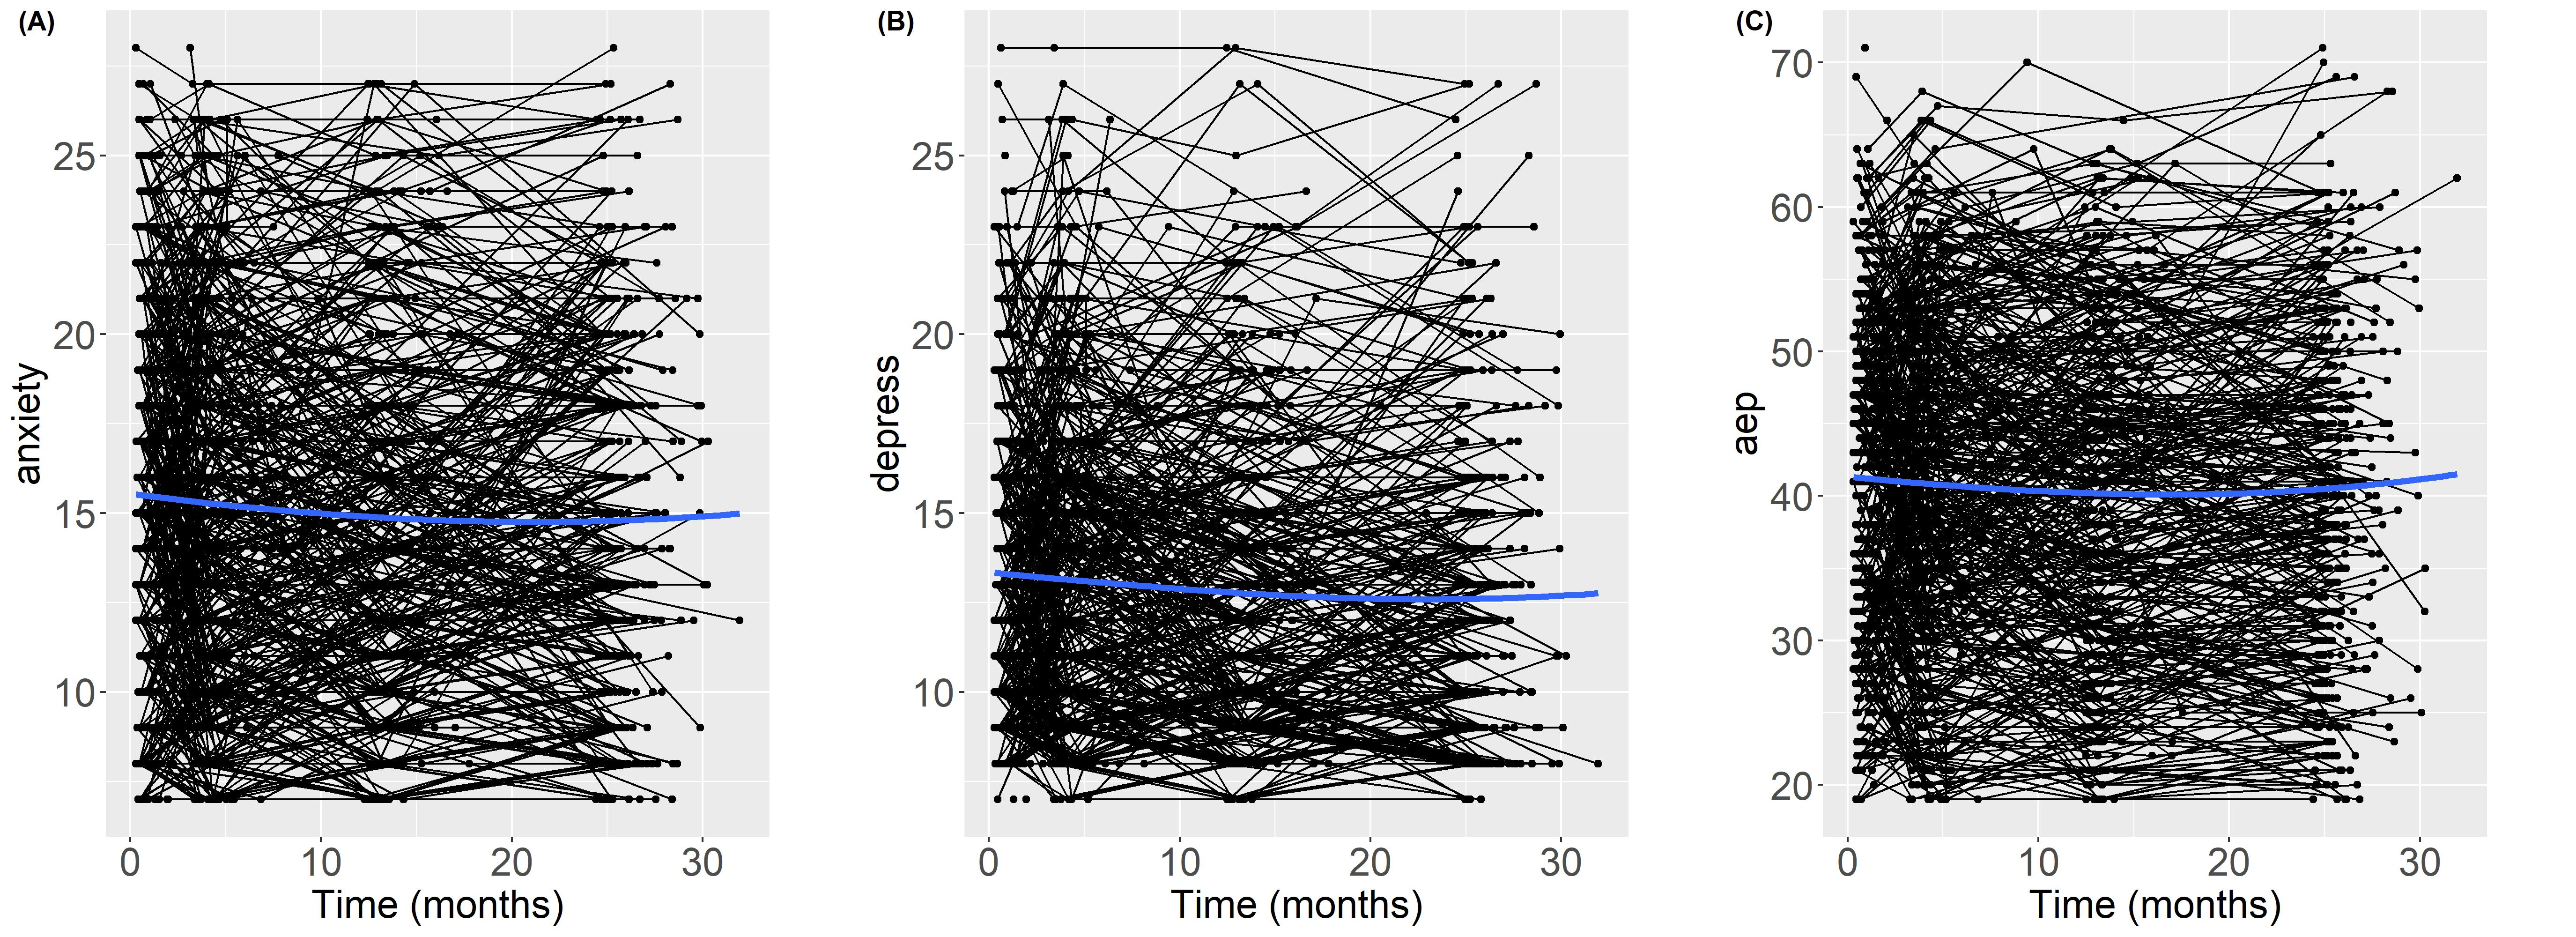
\includegraphics[width=\textwidth,height=5cm]{./Figures/traj.JPEG}
\caption{\label{fig:traj_demo} Longitudinal trajectories of three features for the epileptic.qol dataset. A locally weighted scatterplot smoothing curve is overlaid on each panel to provide an estimate of the overall trend. (A) longitudinal trajectories of Anxiety score (anxiety), (B) longitudinal trajectories of depression score (depress), (C) longitudinal trajectories of Liverpool Adverse Events Profile (aep).}
\end{figure}
For model-based clustering based on a finite mixture model, it is necessary to normalize the data within each feature in order to model the growth pattern, not the level. This is because the level could dominate the sample variability so that the clusters will be mainly determined by the level and will not necessarily be homogeneous in trend \citep{Heggeseth2018}. Therefore, in the current analysis, the three features were normalized using the \textbf{scale} function before entering the model, using the following commands,
\begin{example}
R> epileptic.qol$anxiety_scale <- scale(epileptic.qol$anxiety)
R> epileptic.qol$depress_scale <- scale(epileptic.qol$depress)
R> epileptic.qol$aep_scale <- scale(epileptic.qol$aep)
\end{example}
\subsubsection{Determining the Number of Clusters}
The following codes fit the BCC model with the number of clusters ranging from 2 to 5, i.e., $K = 2, ..., 5$. For each value of $K$, we saved the mean adjusted adherence (alpha.adjust). For each model, we generated 2000 samples and discarded the first 1000 samples. Note that the following part of the codes may be computationally intensive; if users just want to get familiar with the codes and outputs, a smaller number of iterations and burn-in can be used to reduce the computational time, for example, by setting \code{burn.in = 10, per = 1, and max.iter = 20}.
\begin{example}
R> dat <- epileptic.qol
R> alpha.adjust <-  NULL
R> for (k in 2:5){ 
+        fit.BCC <- BCC.multi (
+        mydat = list(dat$anxiety_scale,dat$depress_scale,dat$aep_scale),
+        dist = c("gaussian"),
+        id = list(dat$id),
+        time = list(dat$time),
+        formula = list(y ~ time +  (1|id)),
+        num.cluster = k,
+        burn.in = 1000,   
+        thin = 1,     
+        per = 100,       
+        max.iter = 2000)  
+        alpha.adjust <- c(alpha.adjust, fit.BCC$alpha.adjust) 
+        }
\end{example}
An alternative specification for the \code{formula} argument is  
\begin{example}
    formula = list(y ~ time +  (1|id), y ~ time +  (1|id), y ~ time +  (1|id))
\end{example}
This specification can be used if the users would like to use different functional forms for different features. Each element within the list corresponds to a model for a feature listed in the \code{mydat} argument.  
To compare the model under different numbers of clusters, one can plot the mean adjusted adherence index using the following commands: 
\begin{example}
R> num.cluster <- 2:5
R> plot(num.cluster, alpha.adjust, type = "o",
+        cex.lab = 1.5, cex.axis = 1.5, cex.main = 1.5, lwd = 2,
+        xlab = "Number of Clusters",
+        ylab = "mean adjusted adherence", main="mean adjusted adherence")
\end{example}
\begin{figure}[h]
\centering
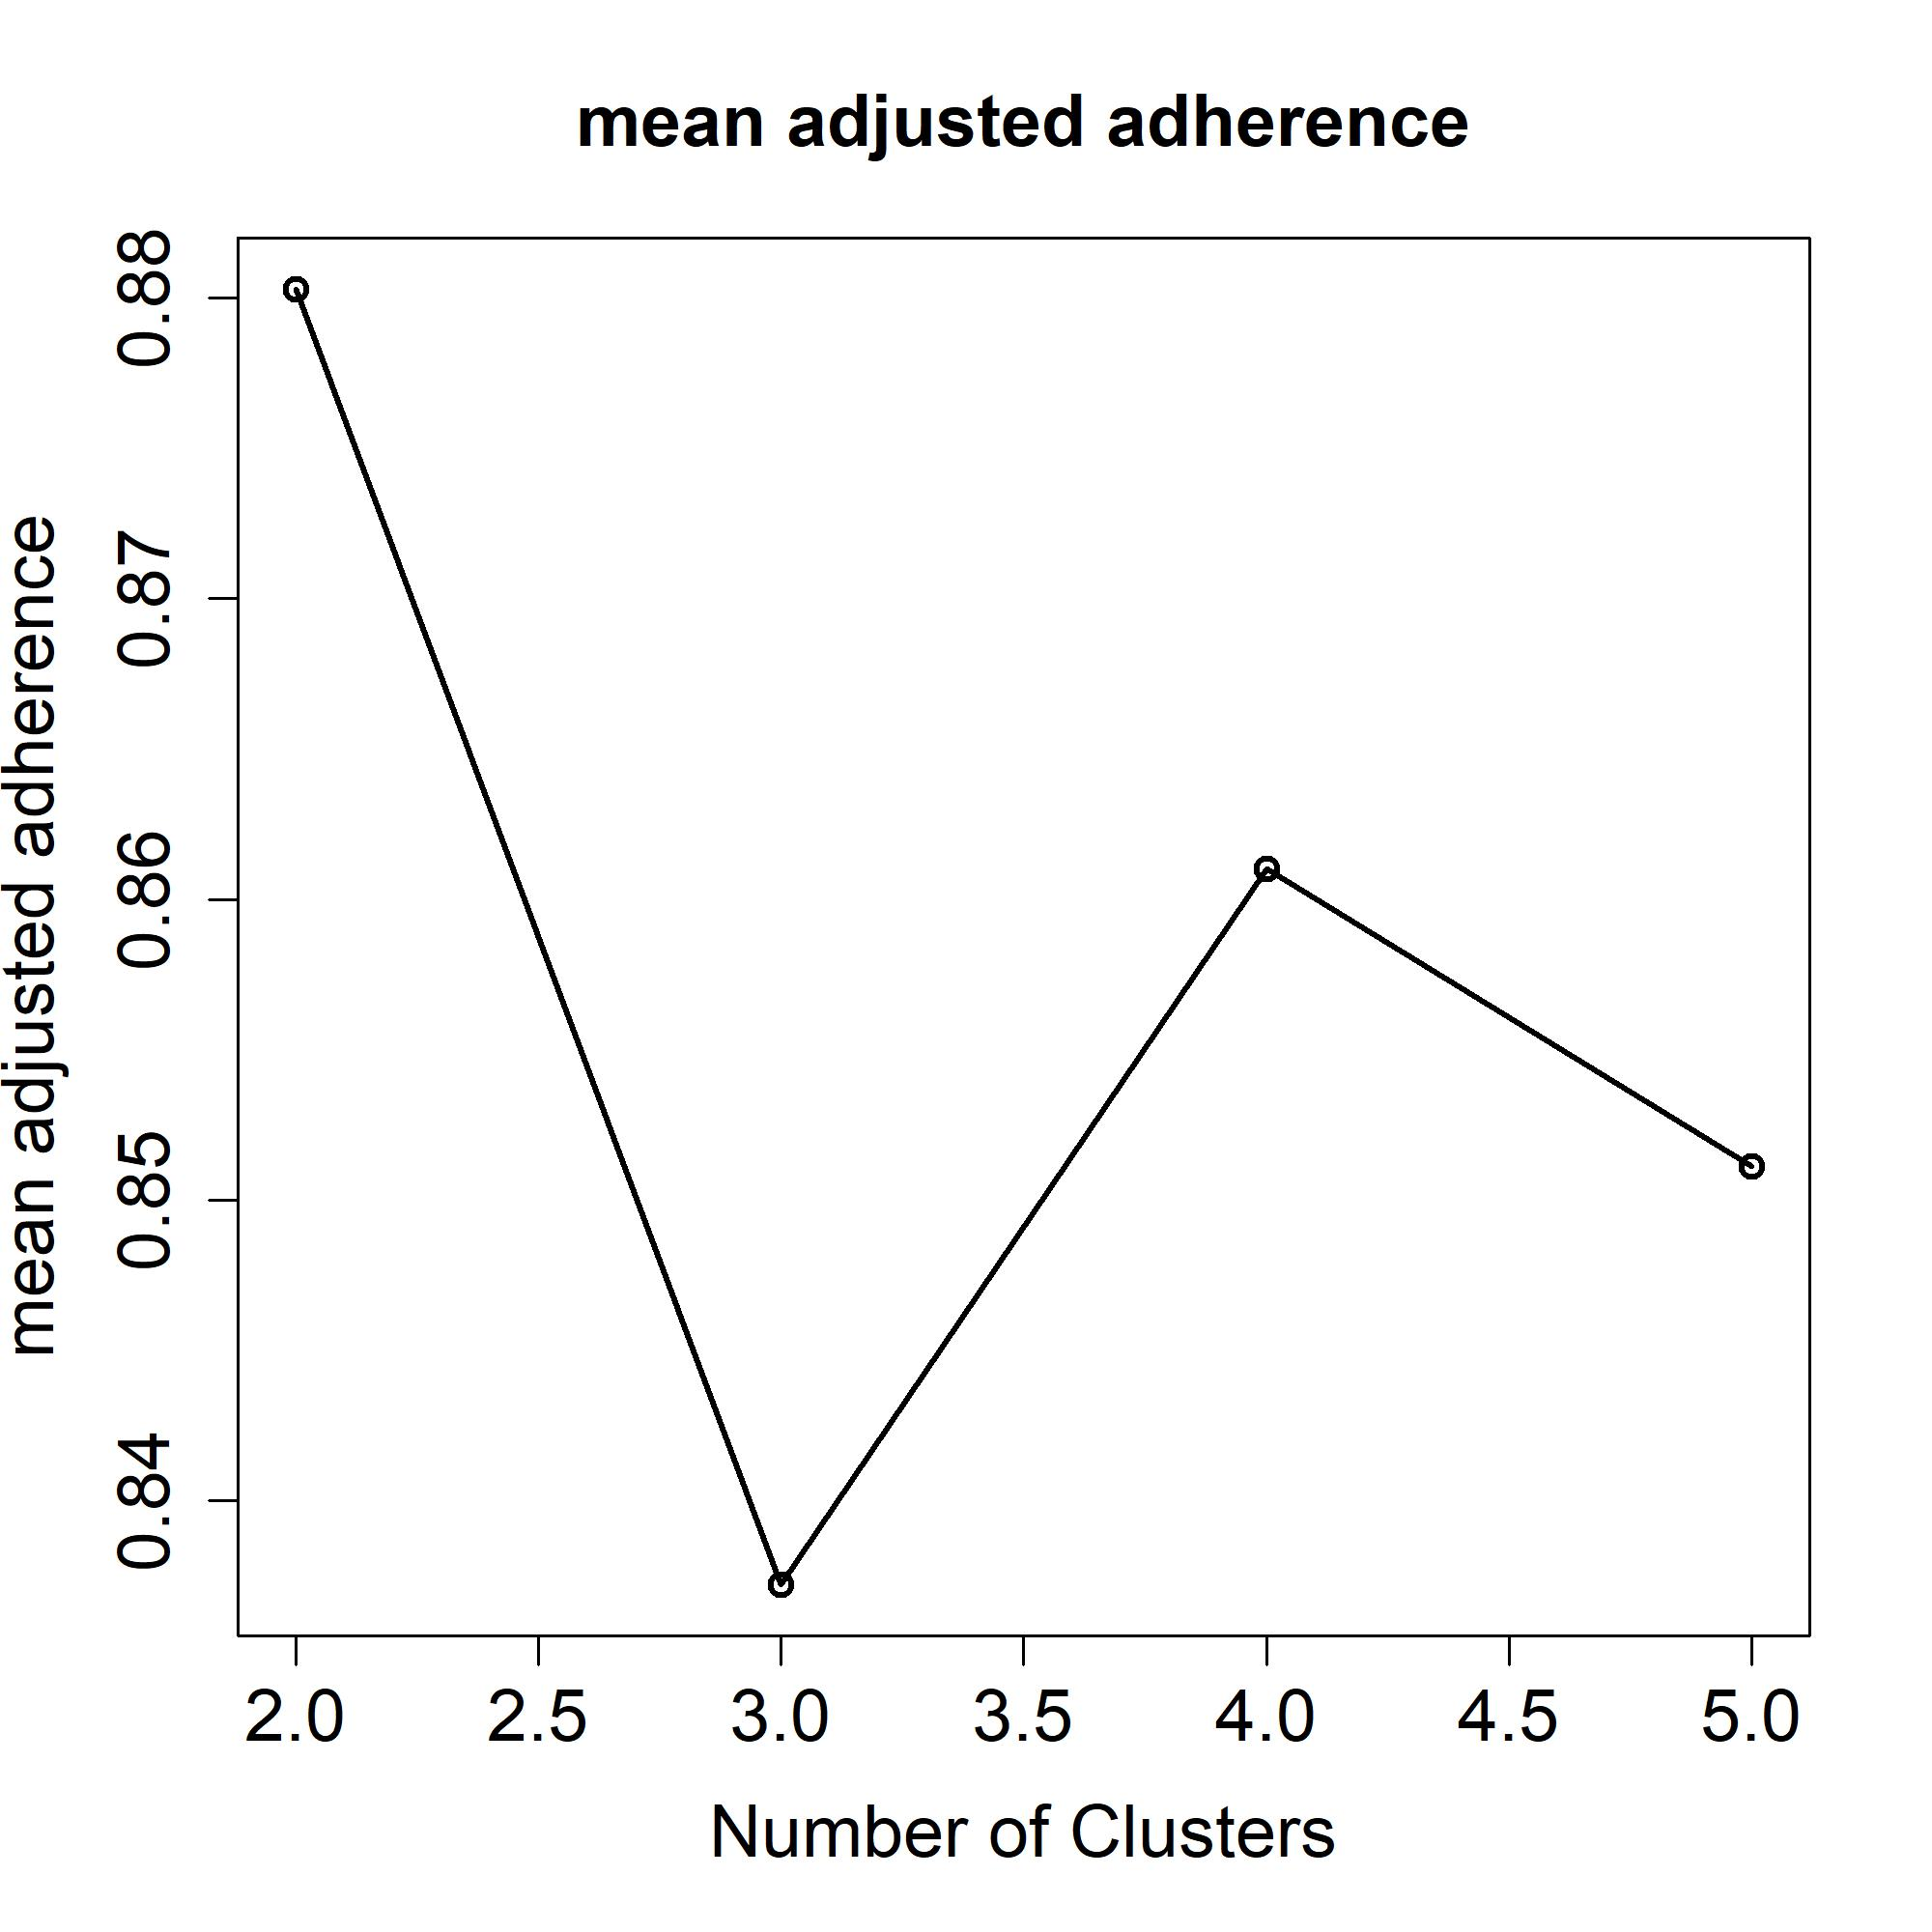
\includegraphics[width=7cm,height=7cm]{./Figures/num_cluster.JPEG}
\caption{\label{fig:num_cluster} Mean adjusted adherence for $K = 2$ to 5 for the epileptic.qol dataset.}
\end{figure}
From Figure \ref{fig:num_cluster}, it was clear that the model with the number of clusters $K=2$ had the largest mean adjusted adherence (0.88), suggesting that a two-cluster model provided the best fit for the data. To determine the number of clusters based on DIC and WAIC, one can also use the \textbf{model.selection.criteria()} function to compute these indices.
Next, we used the following commands to fit the final model with $K=2$. 
\begin{example}
R> fit.BCC2 <- BCC.multi (
+        mydat = list(dat$anxiety_scale, dat$depress_scale, dat$aep_scale),
+        dist = c("gaussian"),
+        id = list(dat$id),
+        time = list(dat$time),
+        formula = list(y ~ time +  (1|id)),
+        num.cluster = 2,
+        burn.in = 1000,   
+        thin = 1,    
+        per = 100,       
+        max.iter = 2000)  
\end{example}
One can apply \code{print()} and \code{summary()} functions to the object returned from \code{BCC.multi()} to obtain summary information of the result, for example, 
\begin{example}
> print(fit.BCC2)
> summary(fit.BCC2)
\end{example} 
Both functions will return result summaries such as the number of individuals, number of features included in the analysis, and tabulation for global and local clusterings. 
\subsubsection{Posterior Summary Statistics and Trace Plots}
One can print the summary statistics for all the model parameters using the following commands (results not shown):
\begin{example}
print(fit.BCC2$summary.stat) 
\end{example} 
As an illustration, we print the estimated cluster probabilities $\boldsymbol{\pi} = (\pi_1, \pi_2)$ as follows: 
\begin{example}
R> print(fit.BCC2$summary.stat$PPI)
\end{example} 
\begin{example}
                   [,1]       [,2]
mean         0.43608373 0.56391627
sd           0.02367214 0.02367214
2.5%         0.39326189 0.51584563
97.5%        0.48415437 0.60673811
geweke.stat -0.78671117 0.78671117
\end{example}
The summary statistics provided the posterior mean, standard deviation (sd), 2.5\%tile, 97.5\%tile, and the Geweke statistics. For example, the posterior mean for $\pi_1$ and $\pi_2$ were 0.44 and 0.56, respectively. This suggested that the estimated cluster proportions for Clusters 1 and 2 are 44\% and 56\%, respectively. The Geweke statistics for $\pi_1$ and $\pi_2$ fell between -2 and 2, suggesting that the two parameters converge to a stationary distribution. 
One can also use the following commands to print the adherence parameters for the three features, i.e., $\boldsymbol{\alpha}=(\alpha_1,\alpha_2,\alpha_3)$:
\begin{example}
R> print(fit.BCC2$summary.stat$ALPHA)
\end{example} 
\begin{example}
                  [,1]       [,2]        [,3]
mean        0.97572877 0.91727462  0.92427049
sd          0.01230074 0.01764104  0.01771331
2.5%        0.94682192 0.88115409  0.88730582
97.5%       0.99620462 0.95091755  0.95581869
geweke.stat 0.10674171 0.05585855 -1.13303537
\end{example}
The output indicated that the posterior means for the adherence parameters were 0.98, 0.92, and 0.92, respectively. This suggested that all three features highly adhered to the global clustering. The Geweke statistics suggested that all the parameters converge to a stationary distribution. One can print similar information for the fixed effect coefficients $\boldsymbol{\gamma}_k$ using commands \code{print(fit.BCC2\$summary.stat\$GA)}, for the variance-covariance matrix of the random effects $\boldsymbol{\Sigma}_k$ using commands \code{print(fit.BCC2\$summary.stat\$SIGMA.SQ.U)}, for the residual variance of continuous features $\boldsymbol{\sigma}_k$ using commands \code{print(fit.BCC2\$summary.stat\$SIGMA.SQ.E)}, for $k=1,...,K$. 
To visualize the MCMC chain for model parameters, one can use the  \textbf{traceplot()} function to generate the trace plots. For example, to generate a trace plot for cluster probabilities $\boldsymbol{\pi} = (\pi_1, \pi_2)$ and the adherence parameters $\boldsymbol{\alpha}=(\alpha_1,\alpha_2,\alpha_3)$, the following commands were used: 
\begin{example}
R> traceplot(fit = fit.BCC2, parameter = "PPI", ylab = "pi", xlab = "MCMC samples")
R> traceplot(fit = fit.BCC2, parameter = "ALPHA", ylab = "alpha", xlab = "MCMC samples")
\end{example} 
\begin{figure}[h]
\centering
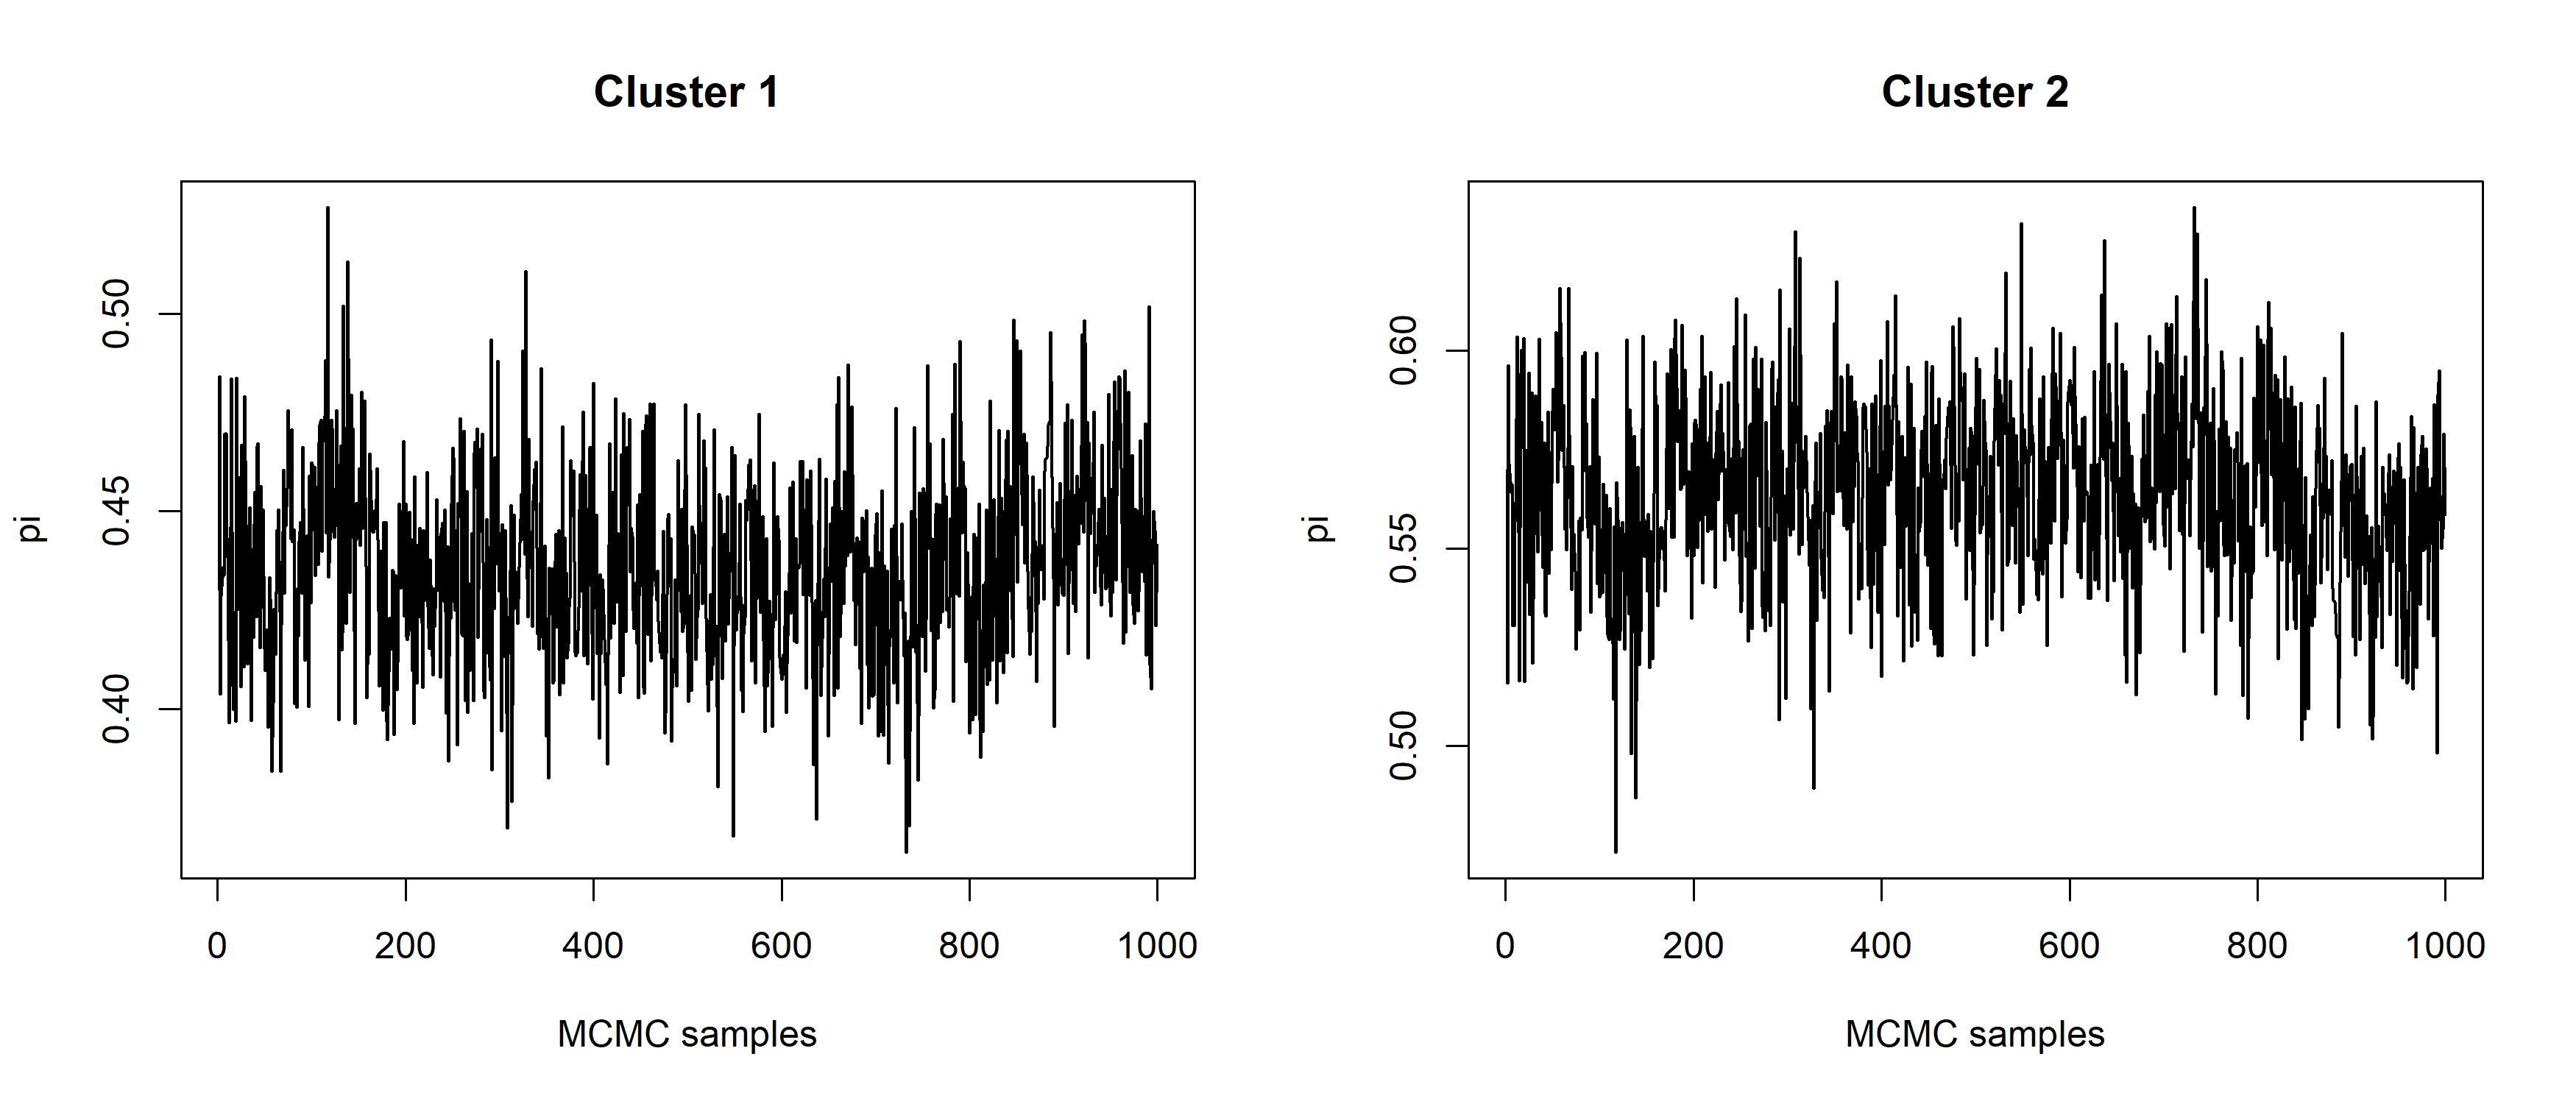
\includegraphics[width=\textwidth,height=6cm]{./Figures/trace_ppi.JPEG}
\caption{\label{fig:trace_ppi}  Trace plots for cluster probabilities $\pi_1$ and $\pi_2$.}
\end{figure}
\begin{figure}[h]
\centering
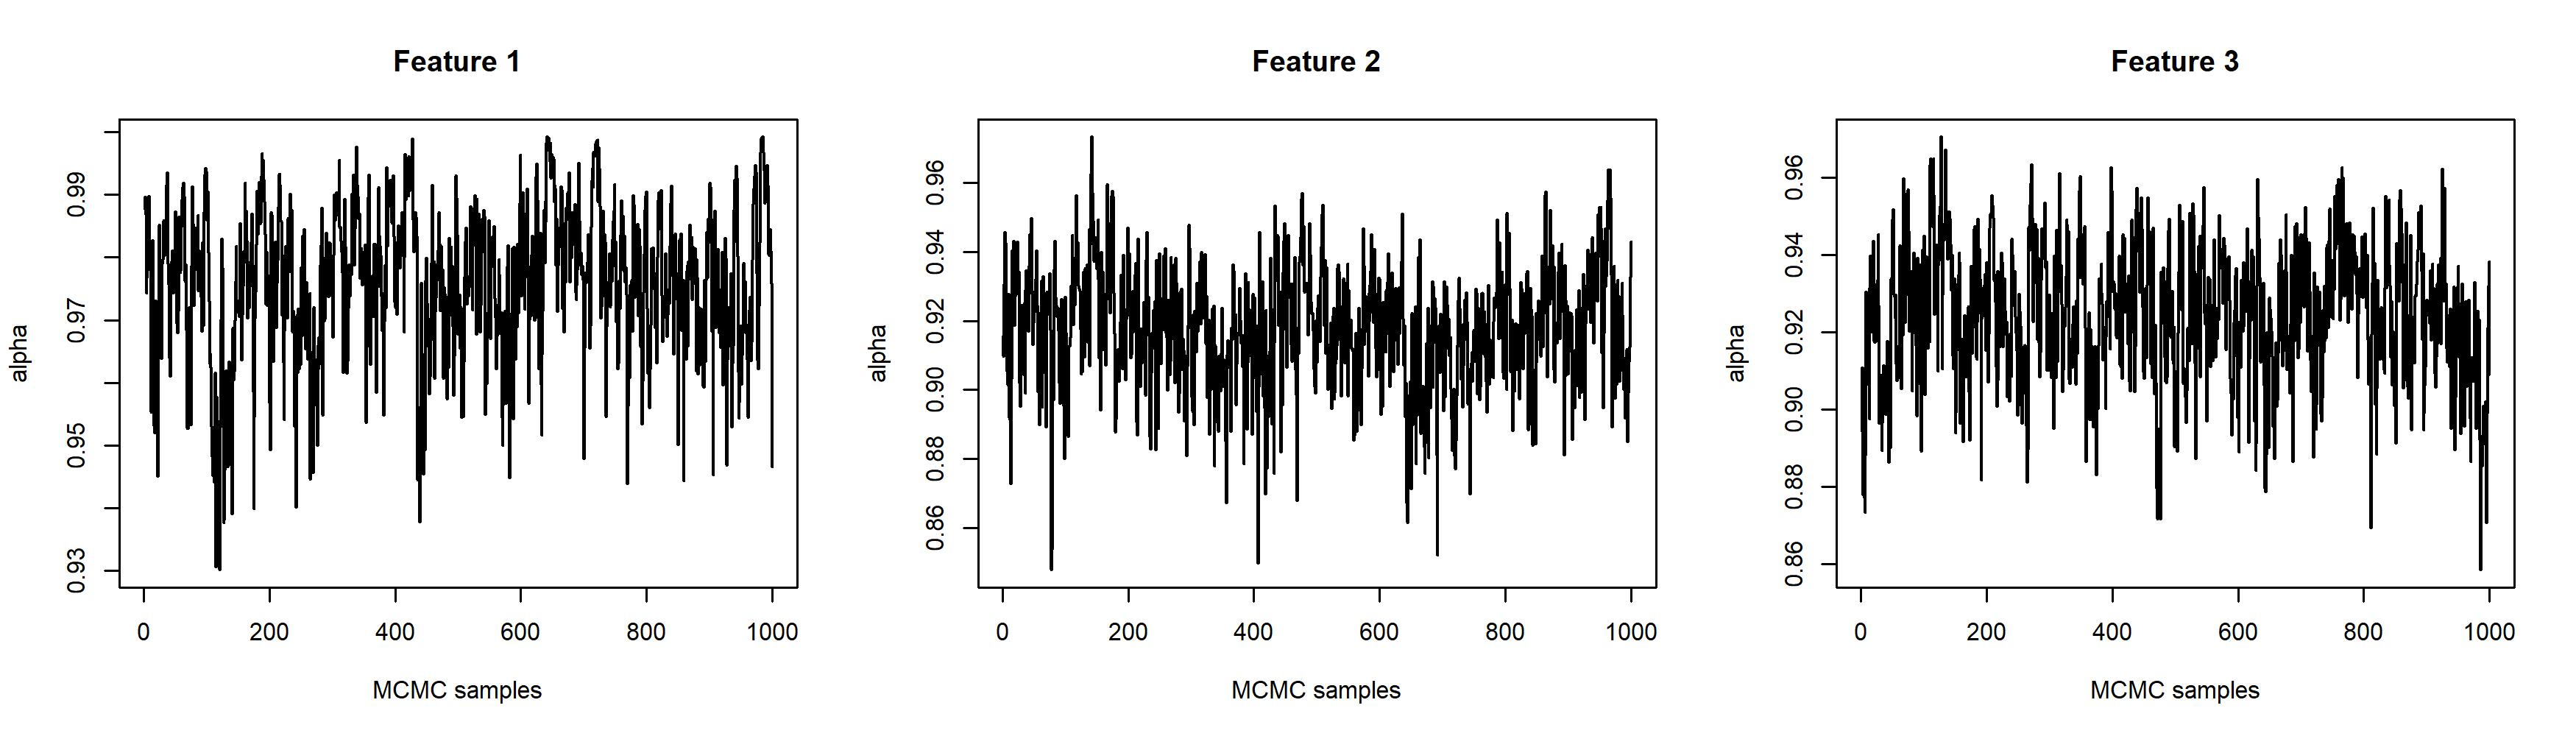
\includegraphics[width=\textwidth,height=6cm]{./Figures/trace_alpha.JPEG}
\caption{\label{fig:trace_alpha}  Trace plots for adherence parameters $\alpha_1$, $\alpha_2$, $\alpha_3$.}
\end{figure}
The outputs are displayed in Figure \ref{fig:trace_ppi} and Figure \ref{fig:trace_alpha}, respectively. These trace plots suggested that $\pi_1$, $\pi_2$, $\alpha_1$, $\alpha_2$, and $\alpha_3$ are mixing well and converging. 
In addition, one can generate trace plots for cluster-specific parameters, for example, the fixed effect regression coefficients, $\boldsymbol{\gamma}_{k, r} = (\boldsymbol{\gamma}_{k, r1}, \boldsymbol{\gamma}_{k, r2})$, with the first element as the intercept and the second element as the slope. The following commands generate trace plots (results not shown) for Cluster 1 of the first feature (anxiety), second (depress), and third (aep) features, that is,  $\boldsymbol{\gamma}_{1,1} = (\gamma_{1,11}, \gamma_{1,12})$,  $\boldsymbol{\gamma}_{1,2} = (\gamma_{1,21}, \gamma_{1,22})$, and $\boldsymbol{\gamma}_{1,3} = (\gamma_{1,31}, \gamma_{1,32})$. 
\begin{example}
R> traceplot(fit = fit.BCC2, cluster.indx = 1, feature.indx = 1,
+        parameter = "GA", ylab = "GA", xlab = "MCMC samples")
R> traceplot(fit = fit.BCC2, cluster.indx = 1, feature.indx = 2,
+        parameter = "GA", ylab = "GA", xlab = "MCMC samples")
R> traceplot(fit = fit.BCC2, cluster.indx = 1, feature.indx = 3,
+        parameter = "GA", ylab = "GA", xlab = "MCMC samples")
\end{example} 
%\begin{figure}[ht!]
%\centering
%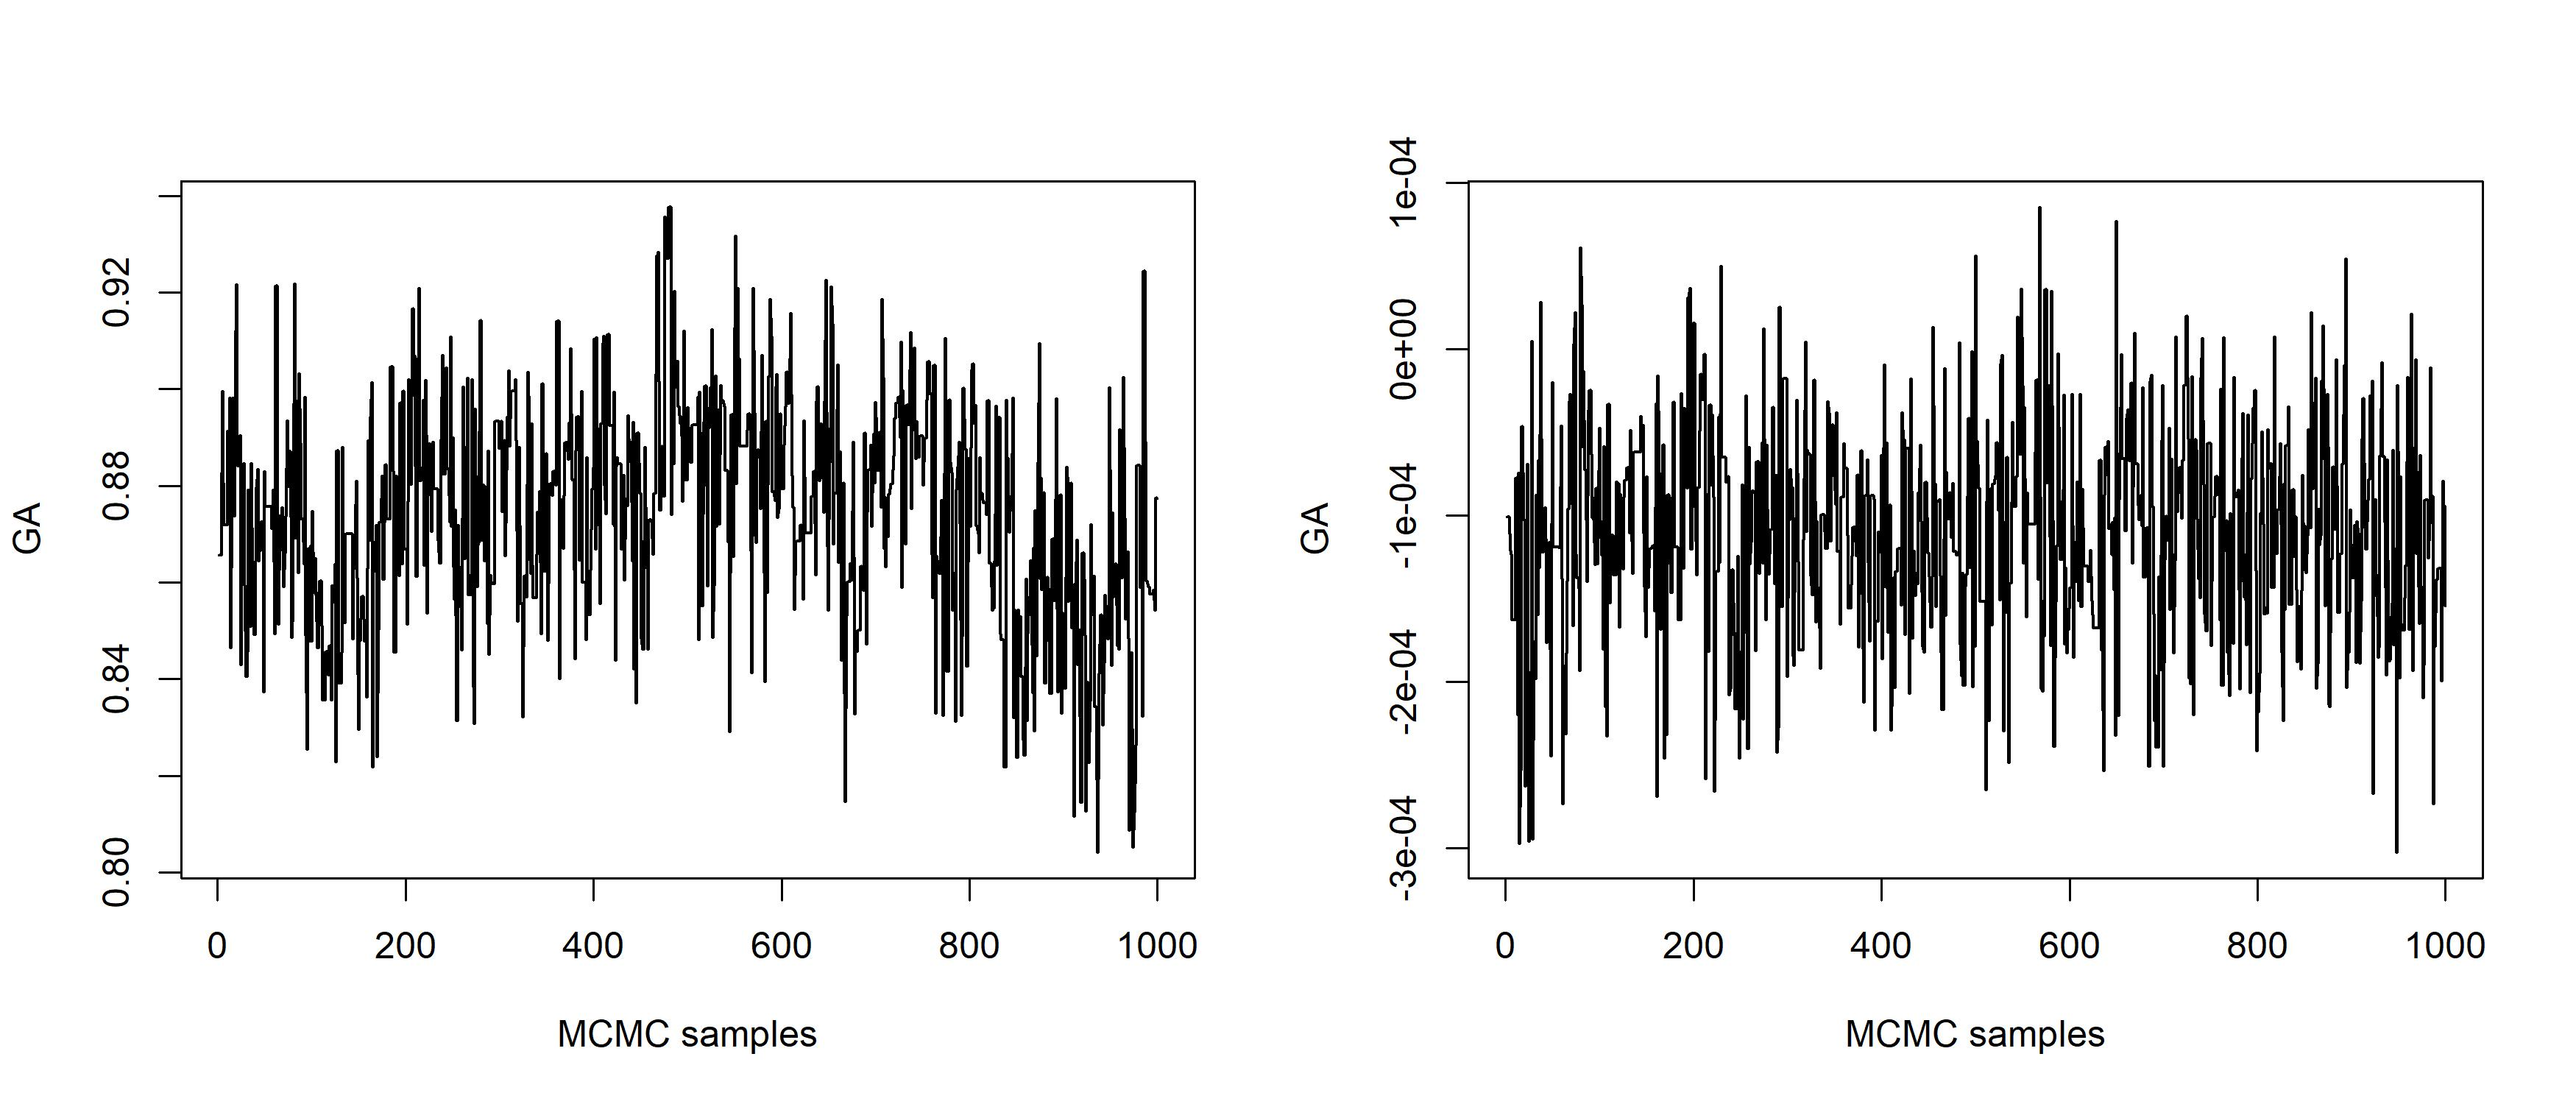
\includegraphics[width=16cm,height=6cm]{./Figures/trace_ga11.JPEG}
%\caption{\label{fig:trace_ga11}  Trace plots for fixed effect coefficients for Cluster 1 of the first feature (anxiety), $\boldsymbol{\gamma}_{1,1} = (\gamma_{1,11}, \gamma_{1,12})$.}
%\end{figure}
%\begin{figure}[ht!]
%\centering
%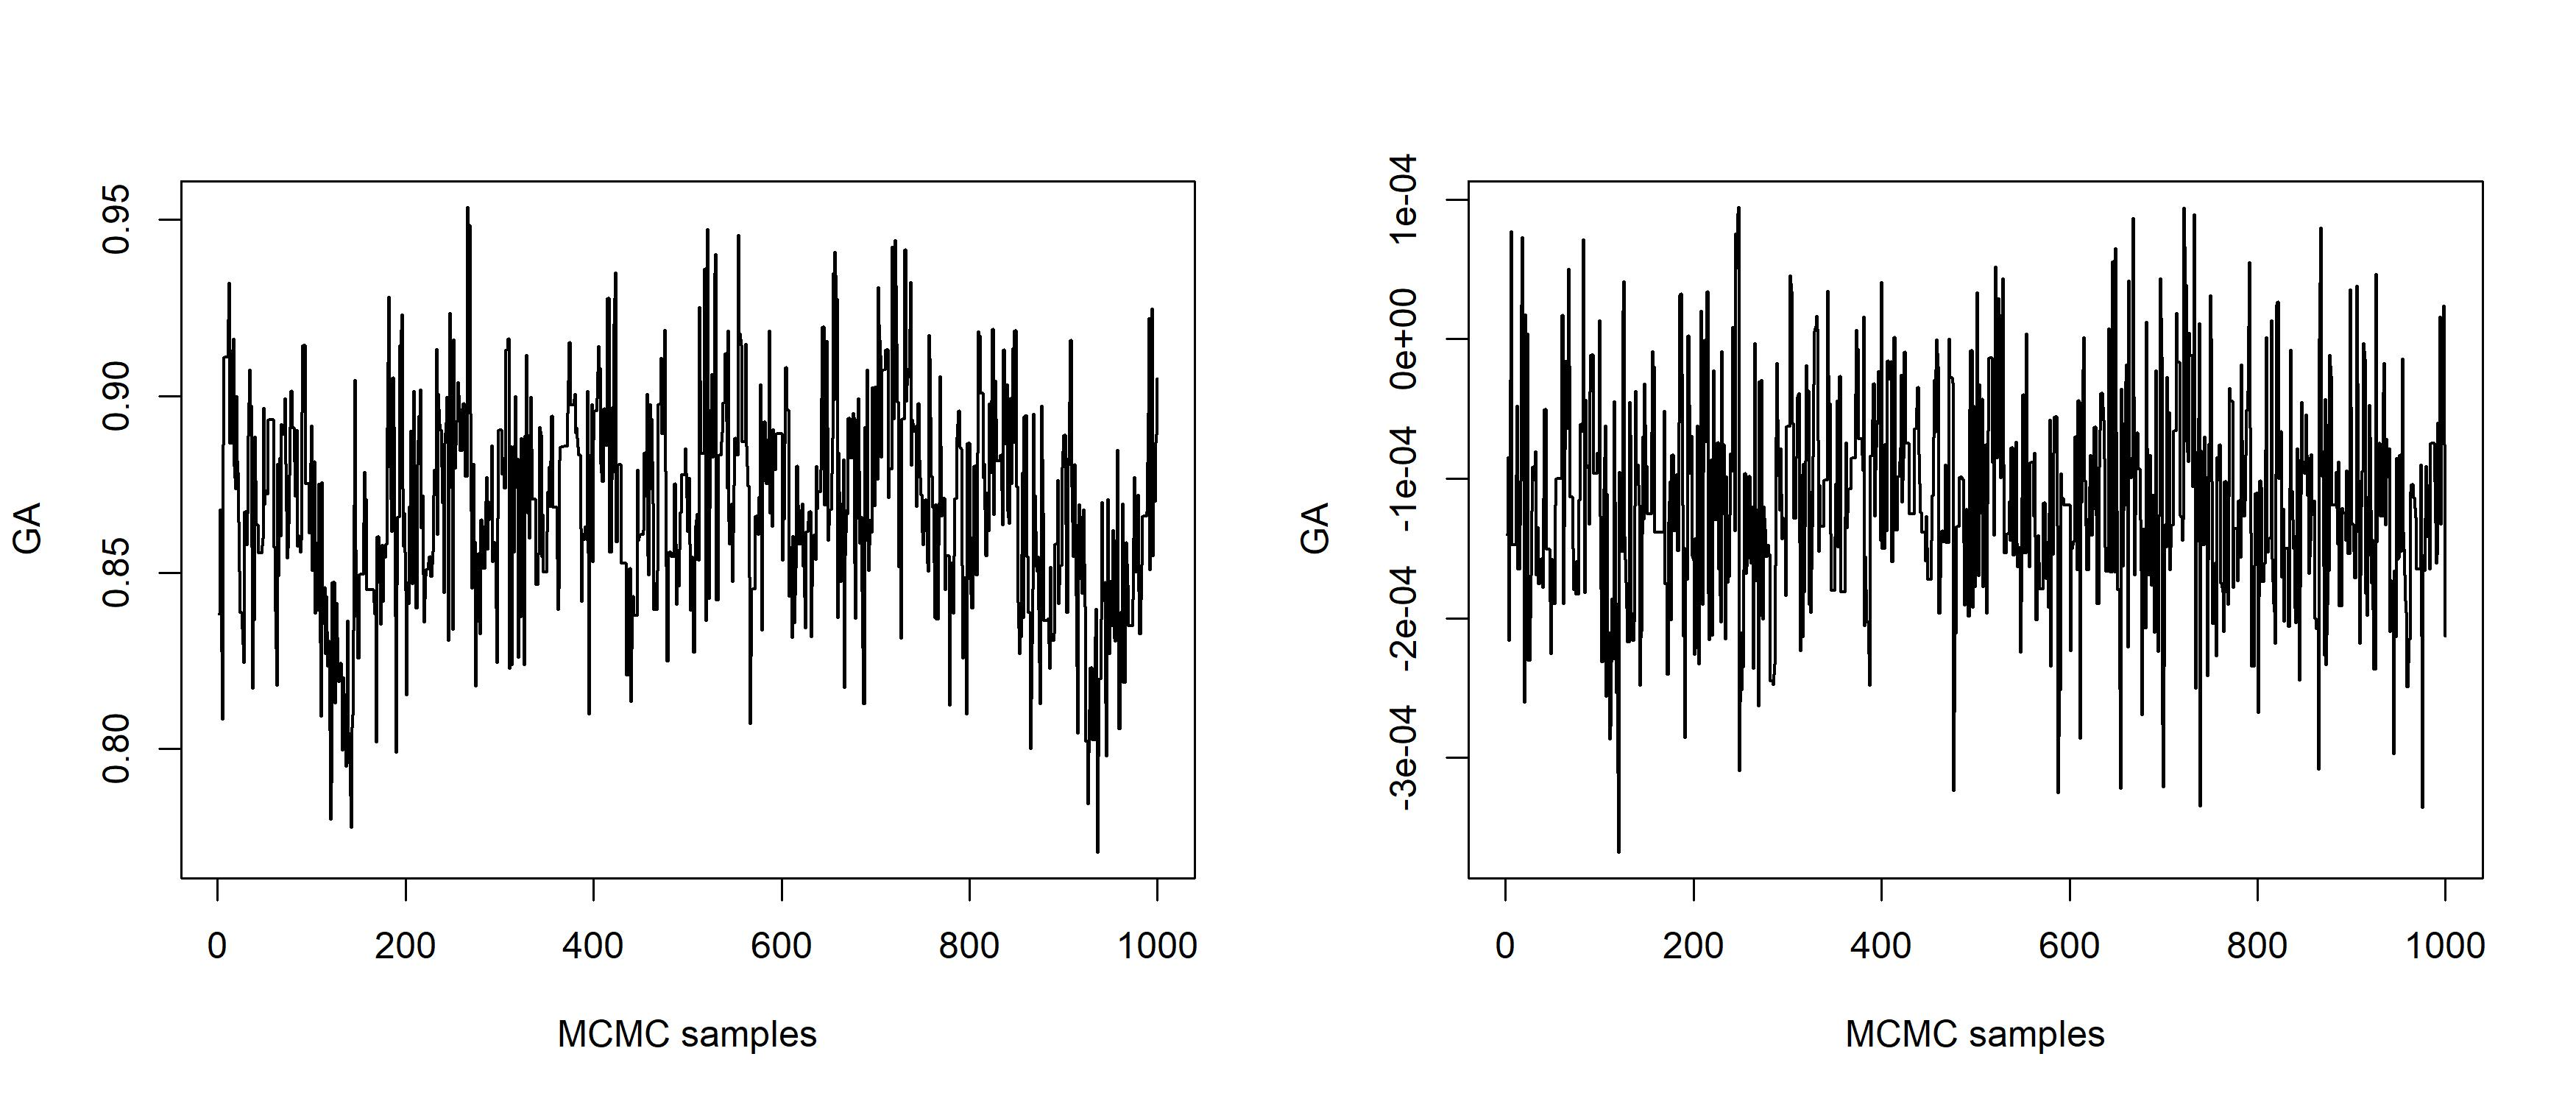
\includegraphics[width=16cm,height=6cm]{./Figures/trace_ga12.JPEG}
%\caption{\label{fig:trace_ga12}  Trace plots for fixed effect coefficients for Cluster 1 of the second feature (depress), $\boldsymbol{\gamma}_{1,2} = (\gamma_{1,21}, \gamma_{1,22})$.}
%\end{figure}
%\begin{figure}[ht!]
%\centering
%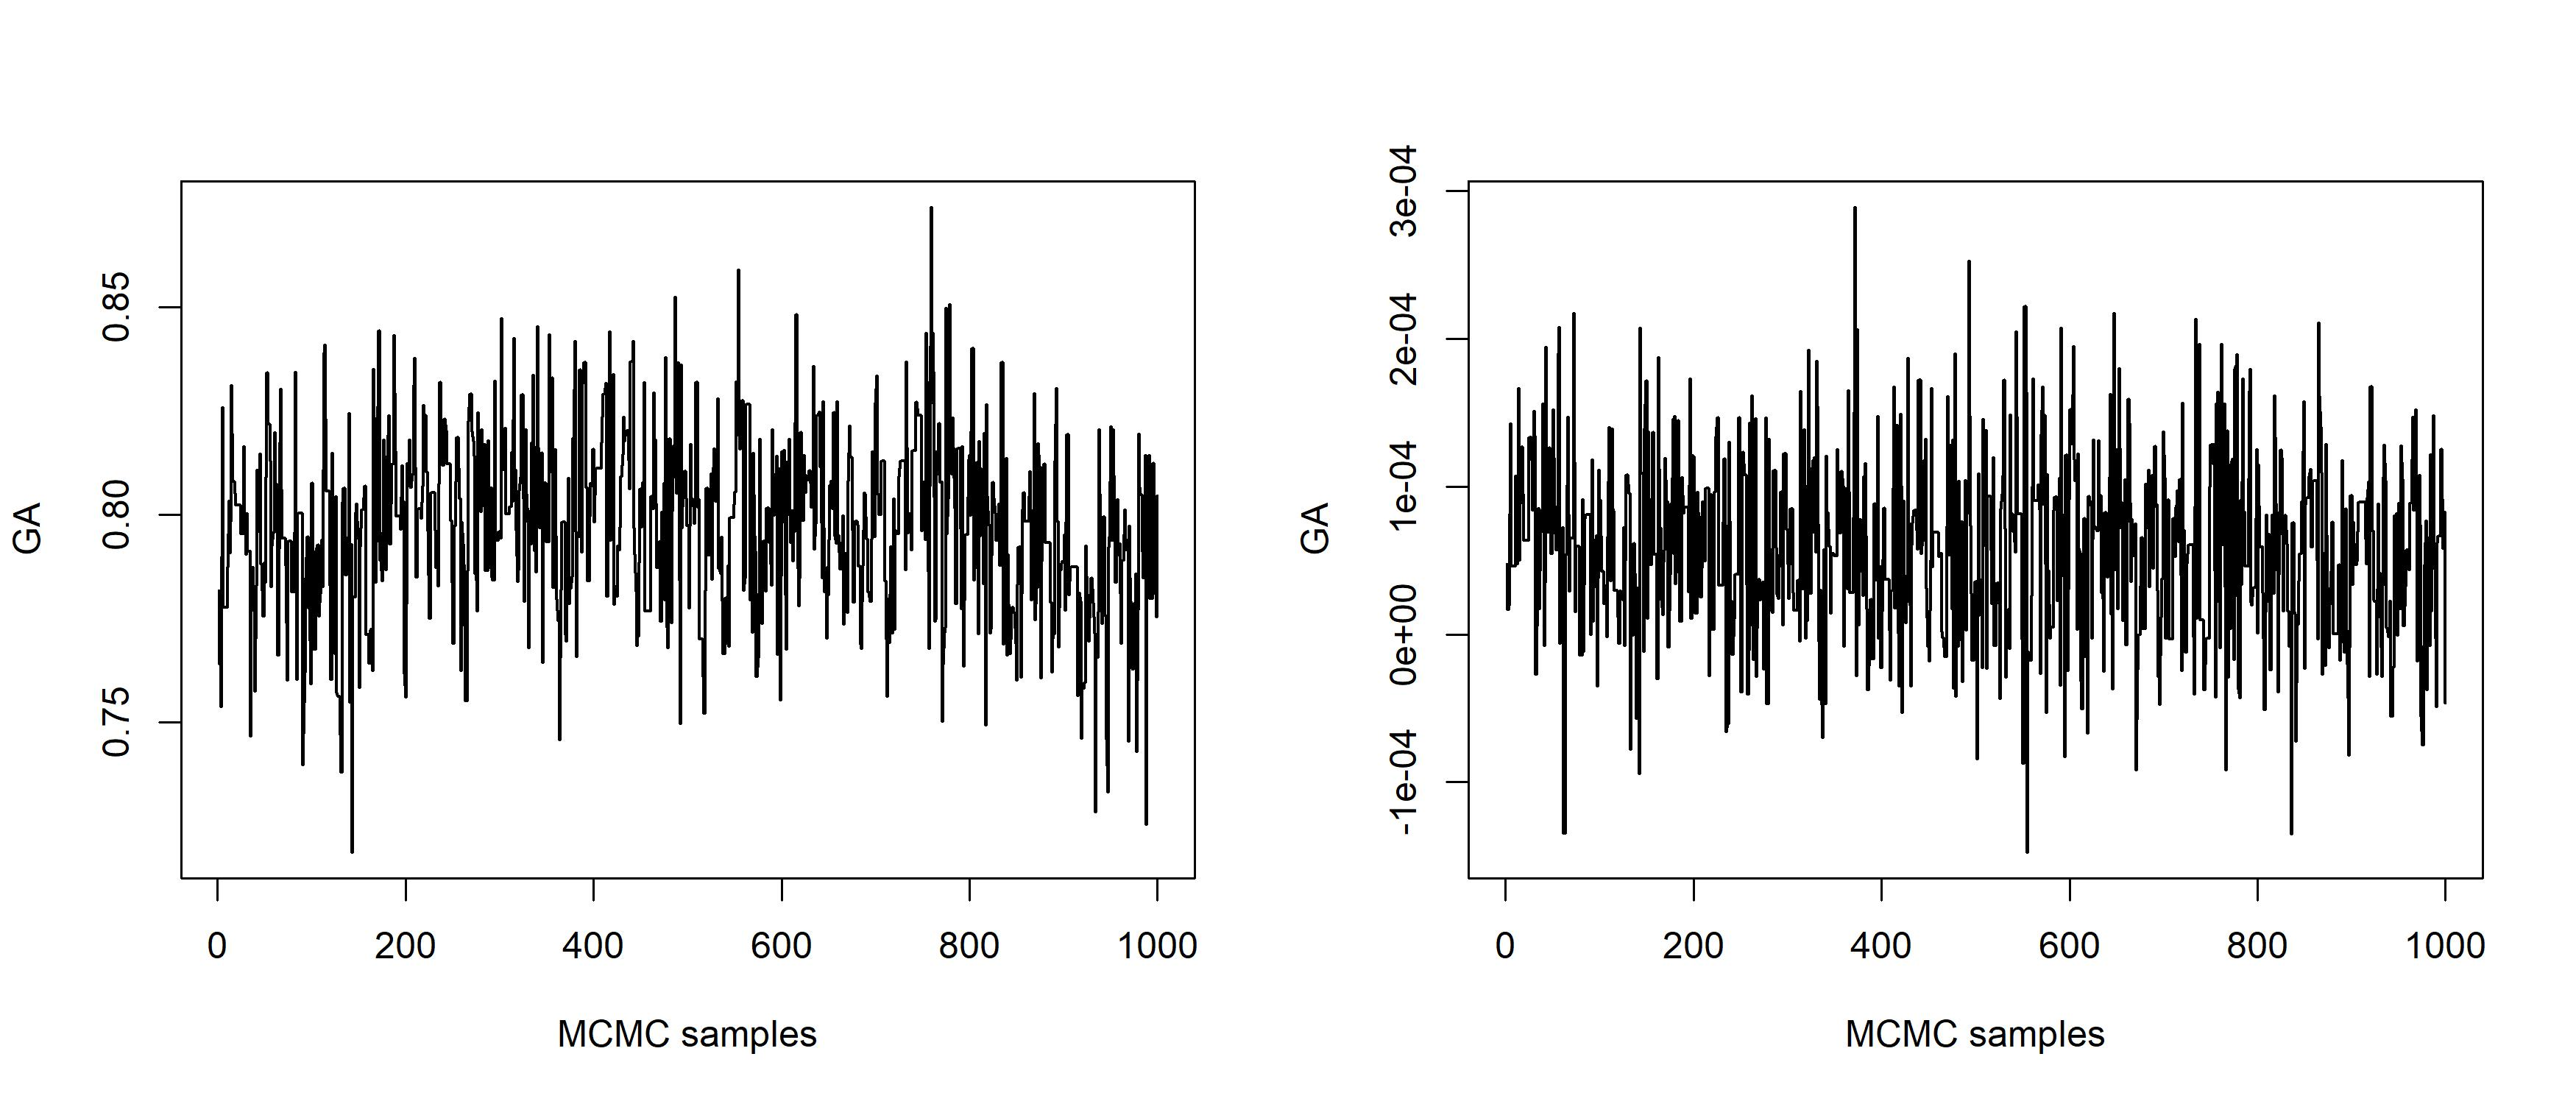
\includegraphics[width=16cm,height=6cm]{./Figures/trace_ga13.JPEG}
%\caption{\label{fig:trace_ga13}  Trace plots for fixed effect coefficients for Cluster 1 of the third feature (aep), $\boldsymbol{\gamma}_{1,3} = (\gamma_{1,31}, \gamma_{1,32})$.}
%\end{figure}
Also, the following commands generated trace plots (results not shown) for Cluster 2 of the first feature (anxiety), second (depress), and third (aep) features, that is,  $\boldsymbol{\gamma}_{2,1} = (\gamma_{2,11}, \gamma_{2,12})$,  $\boldsymbol{\gamma}_{2,2} = (\gamma_{2,21}, \gamma_{2,22})$, and $\boldsymbol{\gamma}_{2,3} = (\gamma_{2,31}, \gamma_{2,32})$. 
\begin{example}
R> traceplot(fit = fit.BCC2, cluster.indx = 2, feature.indx = 1,
+        parameter = "GA", ylab = "GA", xlab="MCMC samples")
R> traceplot(fit = fit.BCC2, cluster.indx = 2, feature.indx = 2,
+        parameter = "GA", ylab = "GA", xlab = "MCMC samples")
R> traceplot(fit = fit.BCC2, cluster.indx = 2, feature.indx = 3,
+        parameter = "GA", ylab = "GA", xlab = "MCMC samples")
\end{example} 
%\begin{figure}[ht!]
%\centering
%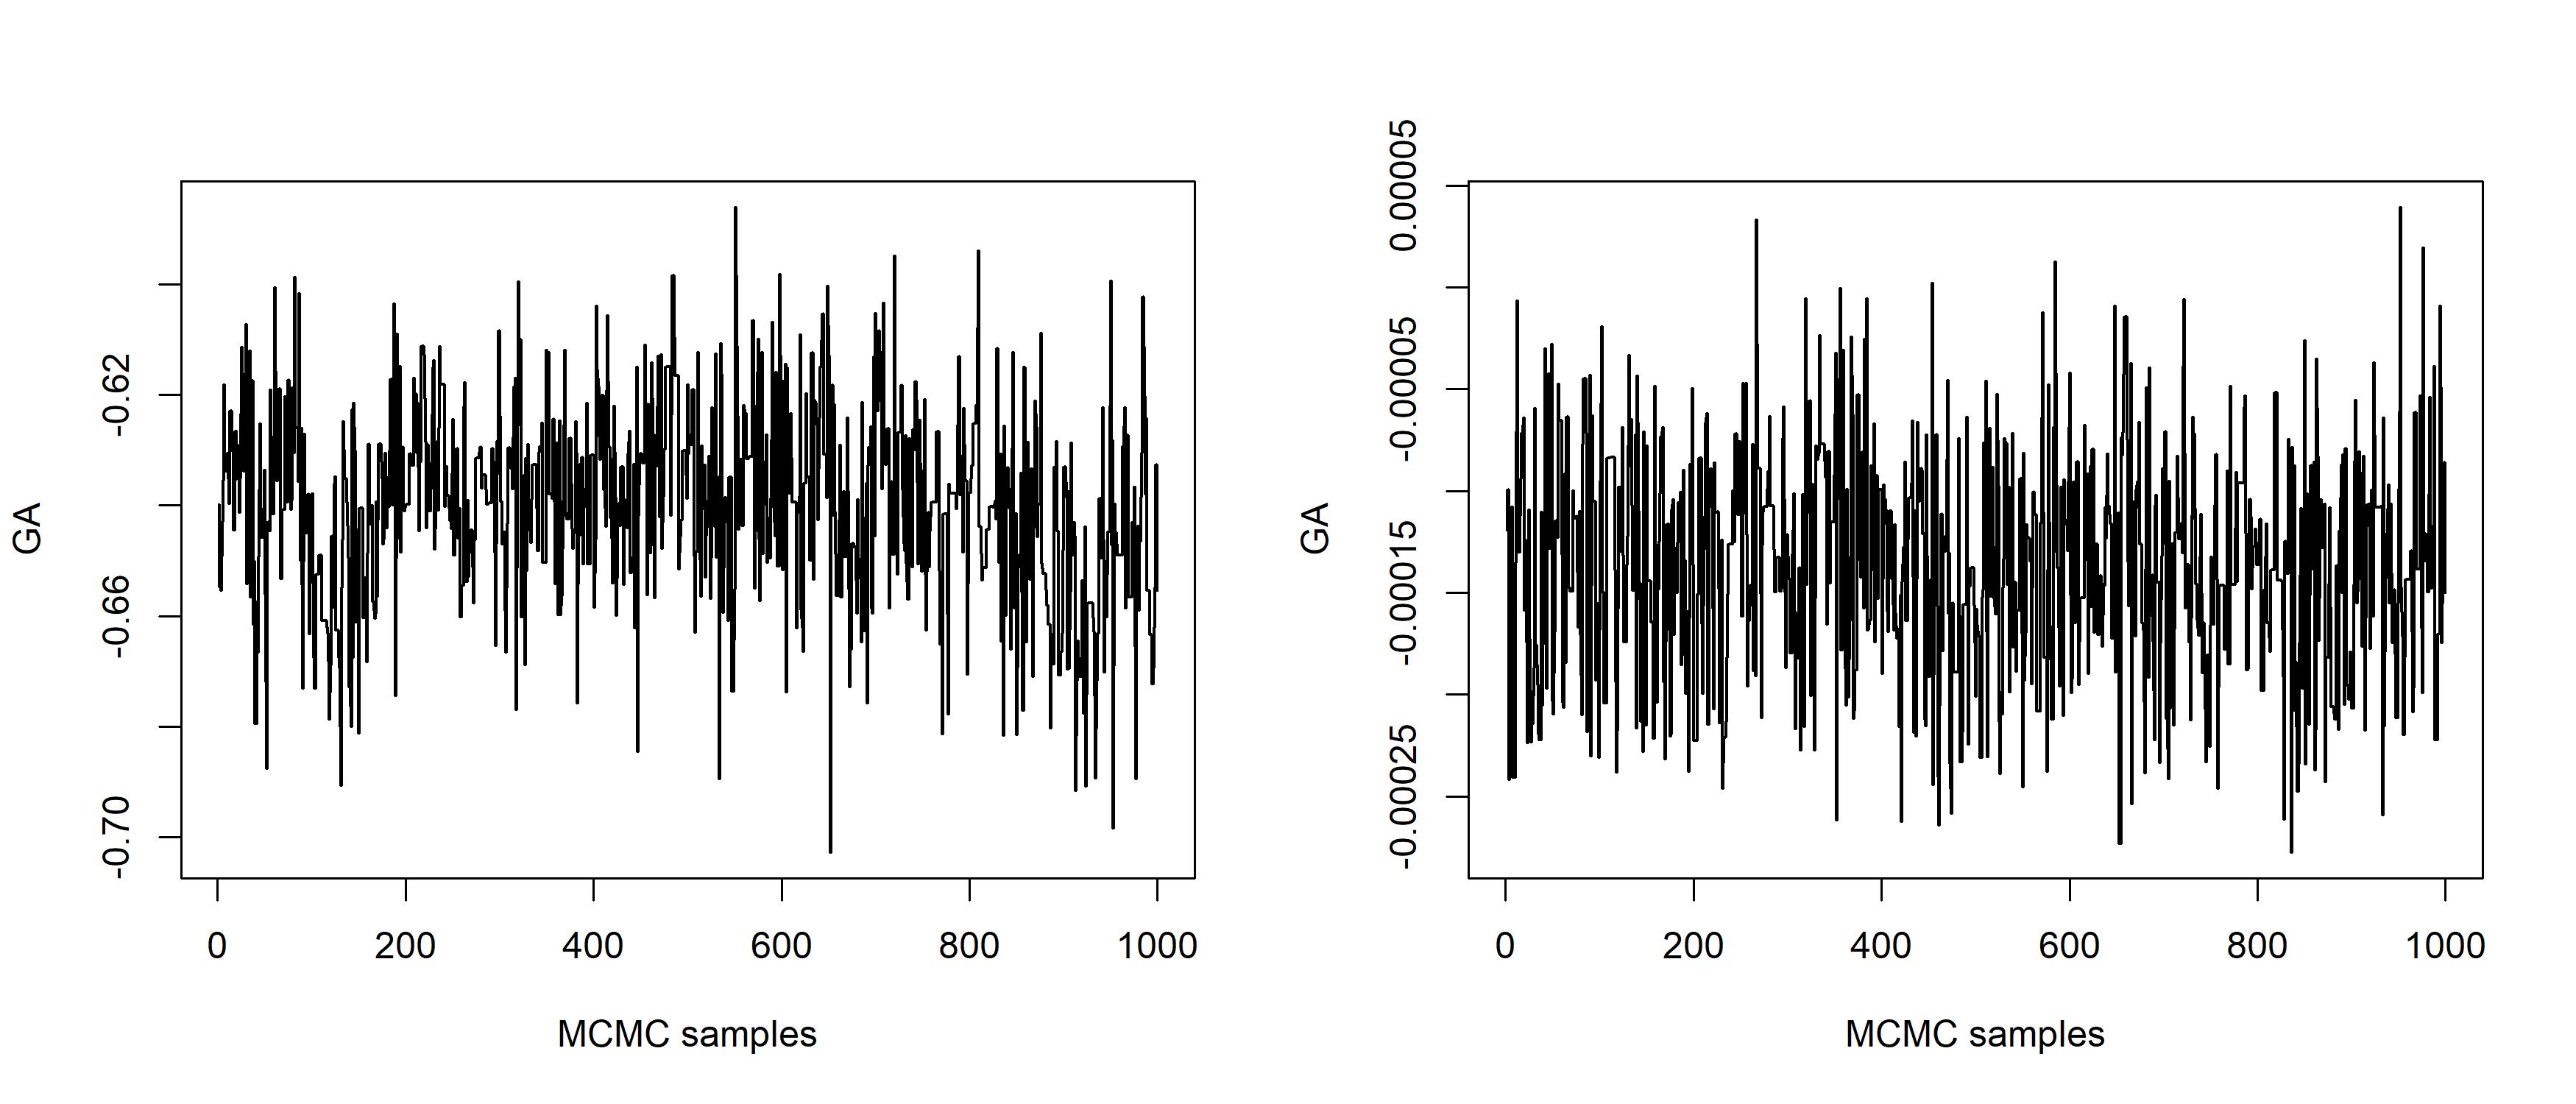
\includegraphics[width=16cm,height=6cm]{./Figures/trace_ga21.JPEG}
%\caption{\label{fig:trace_ga21}  Trace plots for fixed effect coefficients for Cluster 2 of the first feature (anxiety), $\boldsymbol{\gamma}_{2,1} = (\gamma_{2,11}, \gamma_{2,12})$.}
%\end{figure}
%\begin{figure}[ht!]
%\centering
%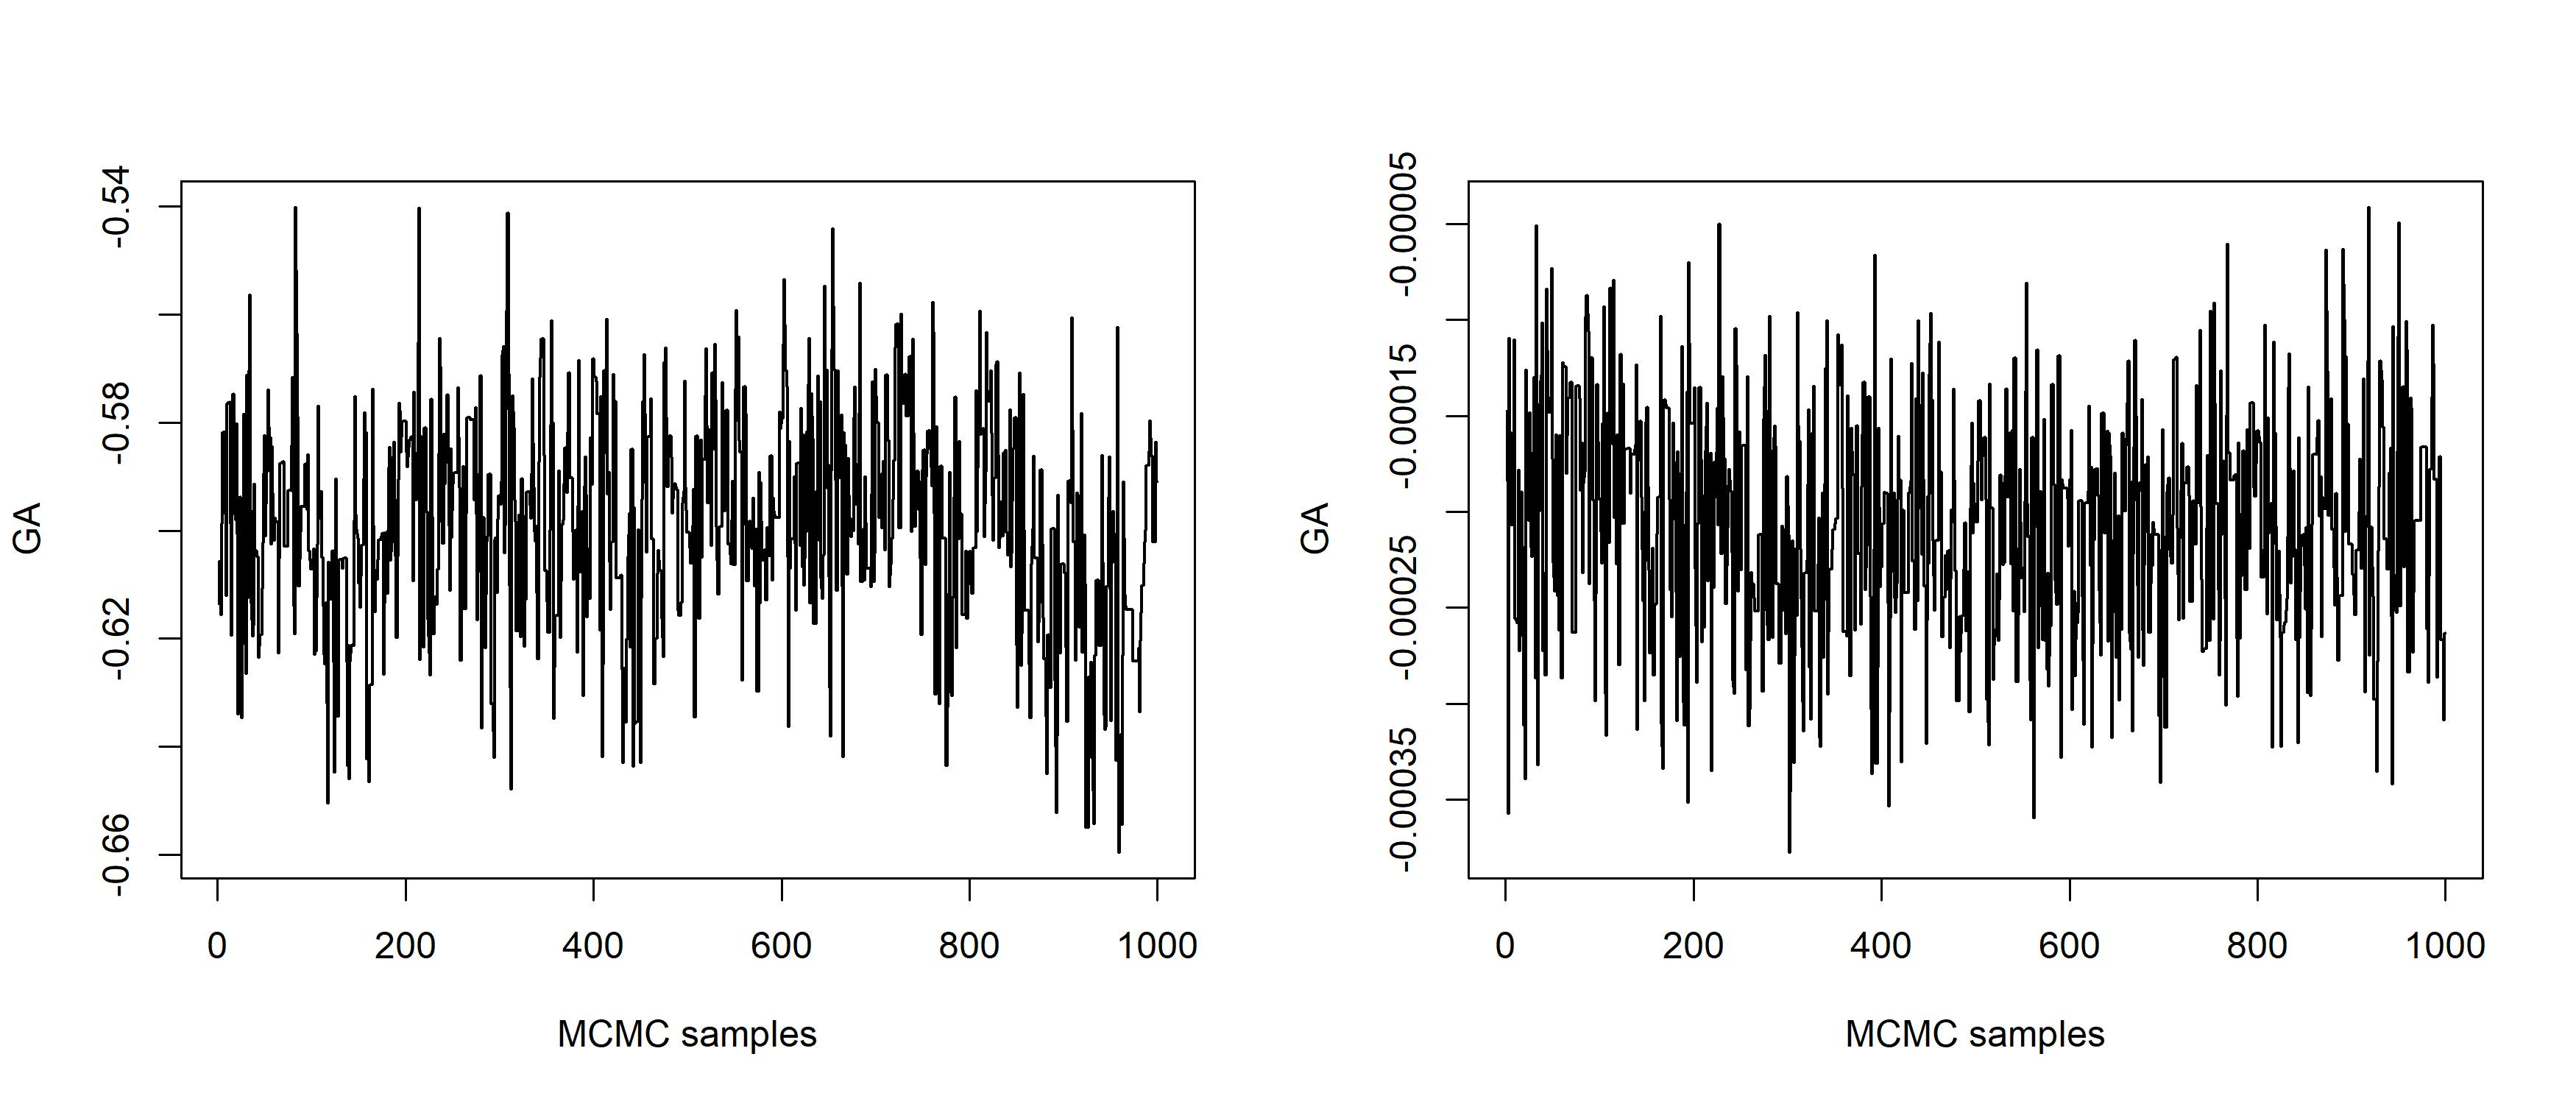
\includegraphics[width=16cm,height=6cm]{./Figures/trace_ga22.JPEG}
%\caption{\label{fig:trace_ga22}  Trace plots for fixed effect coefficients for Cluster 2 of the second feature (depress), $\boldsymbol{\gamma}_{2,2} = (\gamma_{2,21}, \gamma_{2,22})$.}
%\end{figure}
%\begin{figure}[ht!]
%\centering
%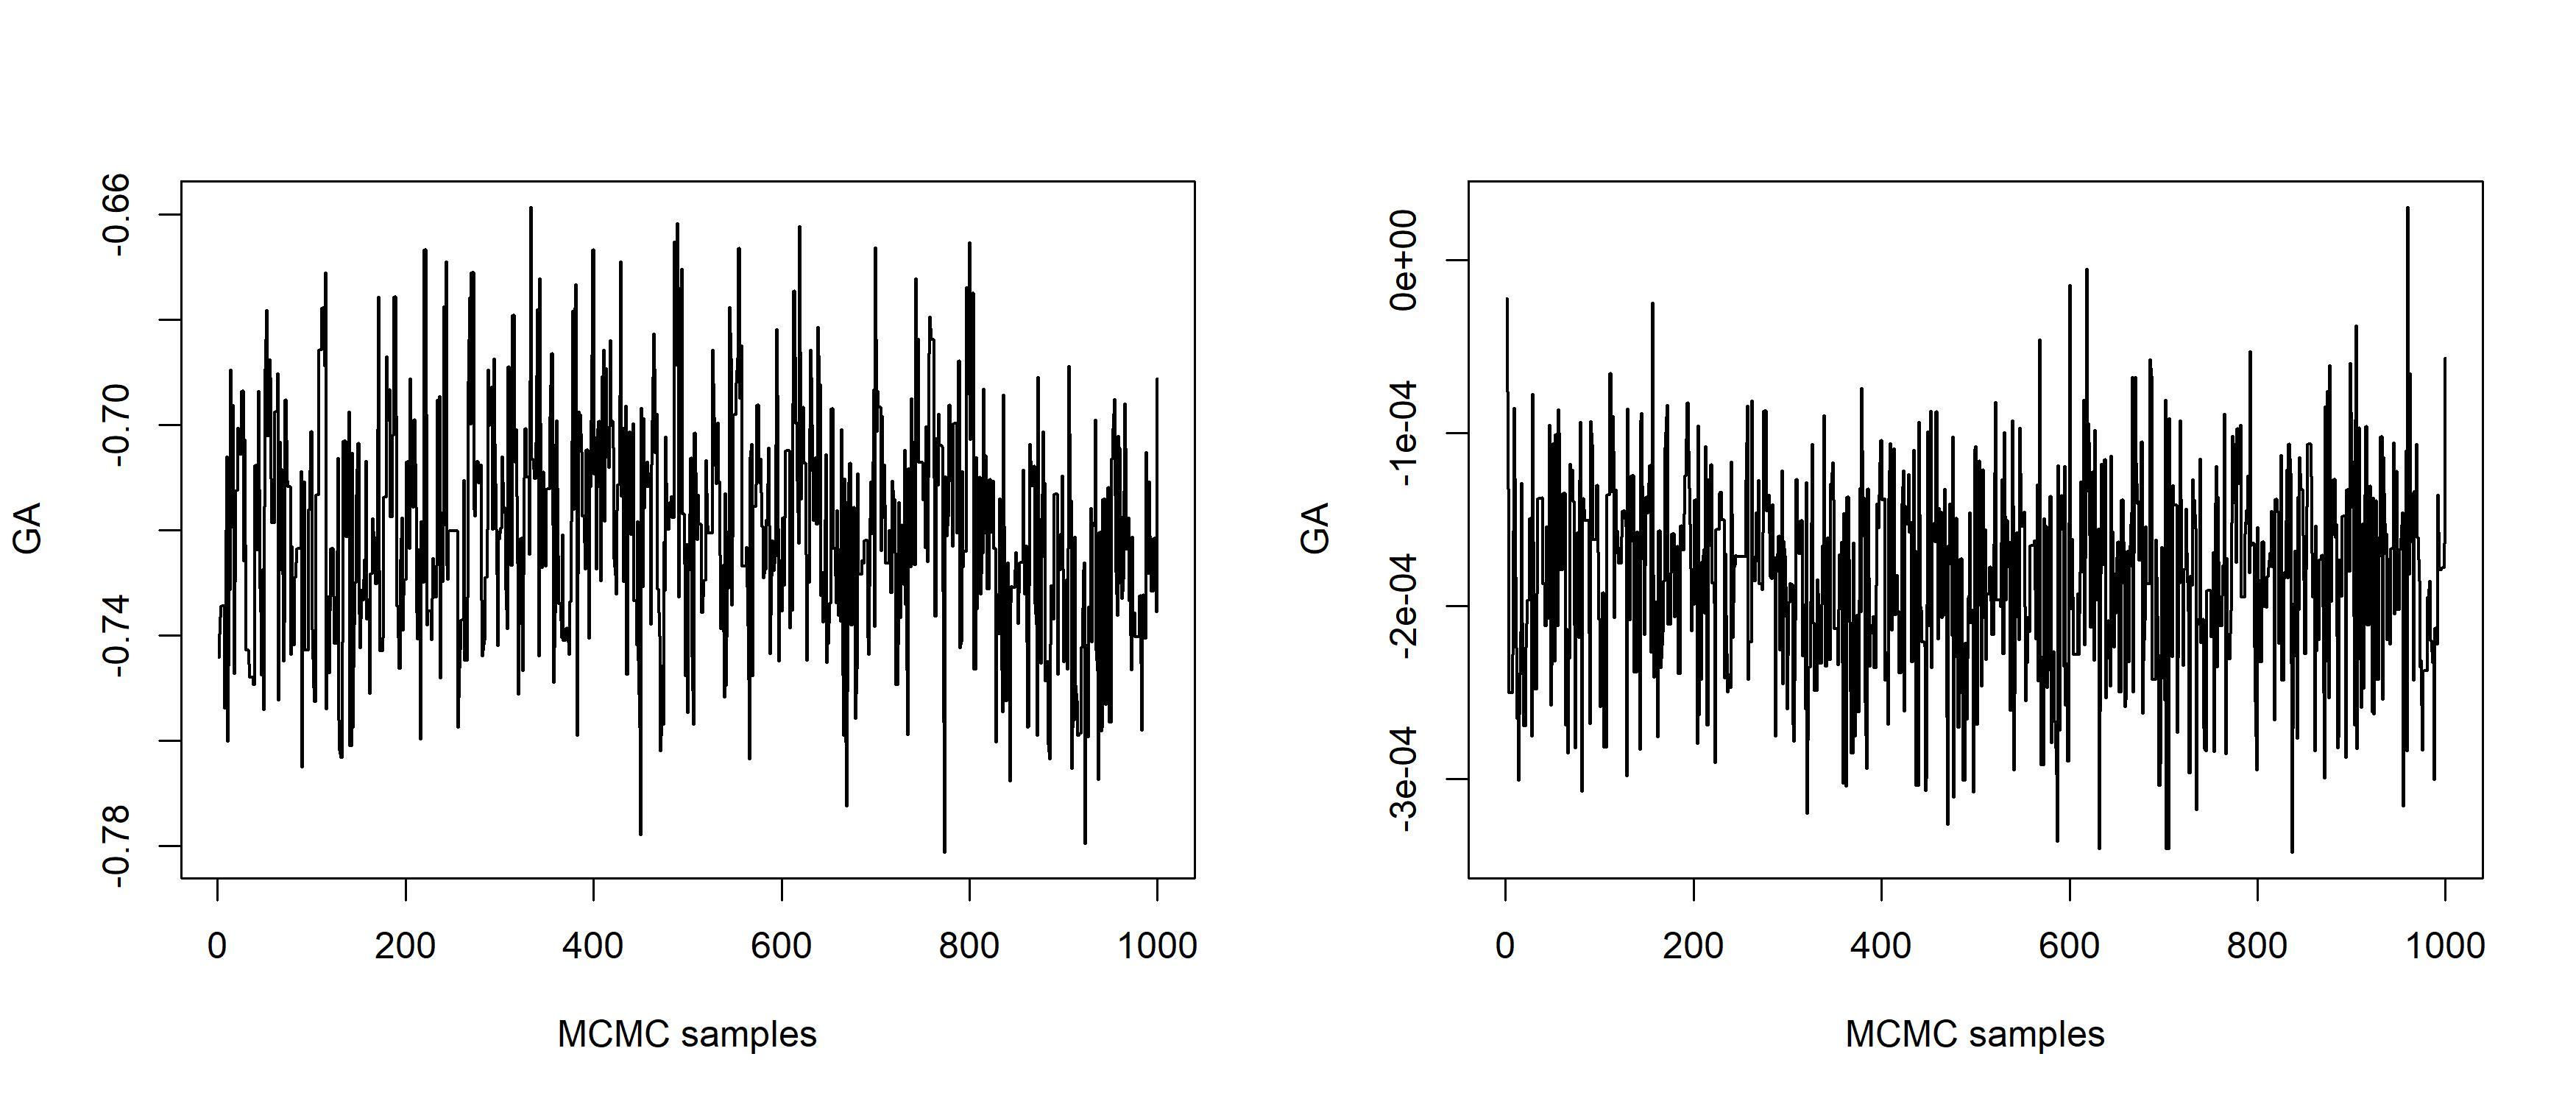
\includegraphics[width=16cm,height=6cm]{./Figures/trace_ga23.JPEG}
%\caption{\label{fig:trace_ga23}  Trace plots for fixed effect coefficients for Cluster 2 of the third feature (aep), $\boldsymbol{\gamma}_{2,3} = (\gamma_{2,31}, \gamma_{2,32})$.}
%\end{figure}
Similarly, one can use \code{parameter = "SIGMA.SQ.U"} to generate the elements of the variance-covariance matrix ($\boldsymbol{\Sigma}_k$) for the random effects, and  \code{parameter = "SIGMA.SQ.E"}  for the residual variance of continuous features $\boldsymbol{\sigma}_k$, for $k=1,...,K$. 
\subsubsection{Longitudinal Profiles by Local and Global Clusters}
The package uses the mode over all the MCMC samples (after burn-in and thinning) as the point estimates for both feature-specific and global clusterings. The following commands computed the number of individuals belonging to each cluster for both feature-specific and global clusterings. 
\begin{example}
R> table(fit.BCC2$cluster.local[[1]])
  1   2 
231 309 
R> table(fit.BCC2$cluster.local[[2]])
  1   2 
223 317  
R> table(fit.BCC2$cluster.local[[3]])
  1   2 
267 273 
R> table(fit.BCC2$cluster.global)
  1   2 
236 304 
\end{example}
That is, for clustering based on the first feature (anxiety) $\boldsymbol{L}_1$, 231 individuals were assigned to Cluster 1 and 309 were assigned to Cluster 2. For clustering based on the second feature (depress) $\boldsymbol{L}_2$, 223 individuals were assigned to Cluster 1 and 317 were assigned to Cluster 2. For clustering based on the third feature (aep) $\boldsymbol{L}_3$, 267 individuals were assigned to Cluster 1 and 273 were assigned to Cluster 2. For global clustering, $\boldsymbol{C}$, 236 individuals were assigned to Cluster 1 and 304 were assigned to Cluster 2.
To plot the longitudinal trajectory of features by local and global clusterings, the \textbf{trajplot()} function can be used. Example codes for plotting the trajectory of the features in the \textbf{epileptic.qol} data are provided as follows: 
\begin{example}
R> gp1 <- trajplot(fit = fit.BCC2, feature.ind = 1,
+        which.cluster = "local.cluster",
+        title= bquote(paste("Local Clustering (",
+        hat(alpha)[1] ==.(round(fit.BCC2$alpha[1],2)),")")),
+        xlab = "time (months)", ylab = "anxiety", color = c("#00BA38", "#619CFF"))
R> gp2 <- trajplot(fit = fit.BCC2, feature.ind = 2,
+        which.cluster = "local.cluster",
+        title = bquote(paste("Local Clustering (",
+        hat(alpha)[2] ==.(round(fit.BCC2$alpha[2],2)),")")),
+        xlab = "time (months)", ylab = "depress", color = c("#00BA38", "#619CFF"))
R> gp3 <- trajplot(fit = fit.BCC2, feature.ind = 3,
+        which.cluster = "local.cluster",
+        title = bquote(paste("Local Clustering (",
+        hat(alpha)[3] ==.(round(fit.BCC2$alpha[3],2)),")")),
+        xlab = "time (months)", ylab = "aep", color = c("#00BA38", "#619CFF"))
R> gp4 <- trajplot(fit = fit.BCC2, feature.ind = 1,
+        which.cluster = "global.cluster",
+        title = "Global Clustering", xlab = "time (months)", ylab = "anxiety", 
+        color = c("#00BA38", "#619CFF"))
R> gp5 <- trajplot(fit = fit.BCC2, feature.ind = 2,
+        which.cluster = "global.cluster",
+        title = "Global Clustering", xlab = "time (months)", ylab = "depress", 
+        color = c("#00BA38", "#619CFF"))
R> gp6 <- trajplot(fit = fit.BCC2, feature.ind = 3,
+        which.cluster = "global.cluster",
+        title = "Global Clustering", xlab = "time (months)", ylab = "aep", 
+        color = c("#00BA38", "#619CFF"))
\end{example} 
The \pkg{cowplot} package \citep{Wilke2019} is used here to combine all six plots together into one figure. 
\begin{example}
R> library("cowplot")
R> dev.new(width = 180, height = 120)
R> plot_grid(gp1, gp2, gp3, gp4, gp5, gp6, 
+        labels = c("(A)", "(B)", "(C)", "(D)", "(E)", "(F)"), 
+        ncol = 3, align = "v" )  
\end{example}
The results are displayed in Figure \ref{fig:traj_epileptic_qol}. The top panel (A, B, and C) shows the three features plotted by local clustering indices, whereas the bottom panel (D, E, F) shows the three features plotted by global clustering indices. Individuals in Cluster 1 had lower anxiety scores, depression scores, and aep scores, which represented a better health condition compared to those in Cluster 2. The local clustering based on the anxiety score highly adhered to the global clustering ($\hat{\alpha}_1 = 0.98$), followed by aep ($\hat{\alpha}_2 = 0.92$) and depress scores ($\hat{\alpha}_3 = 0.92$), respectively. This suggested that all three features highly adhered to the global clustering, and the anxiety score contributed the most information to determine the global clustering. 
\begin{figure}[h]
\centering
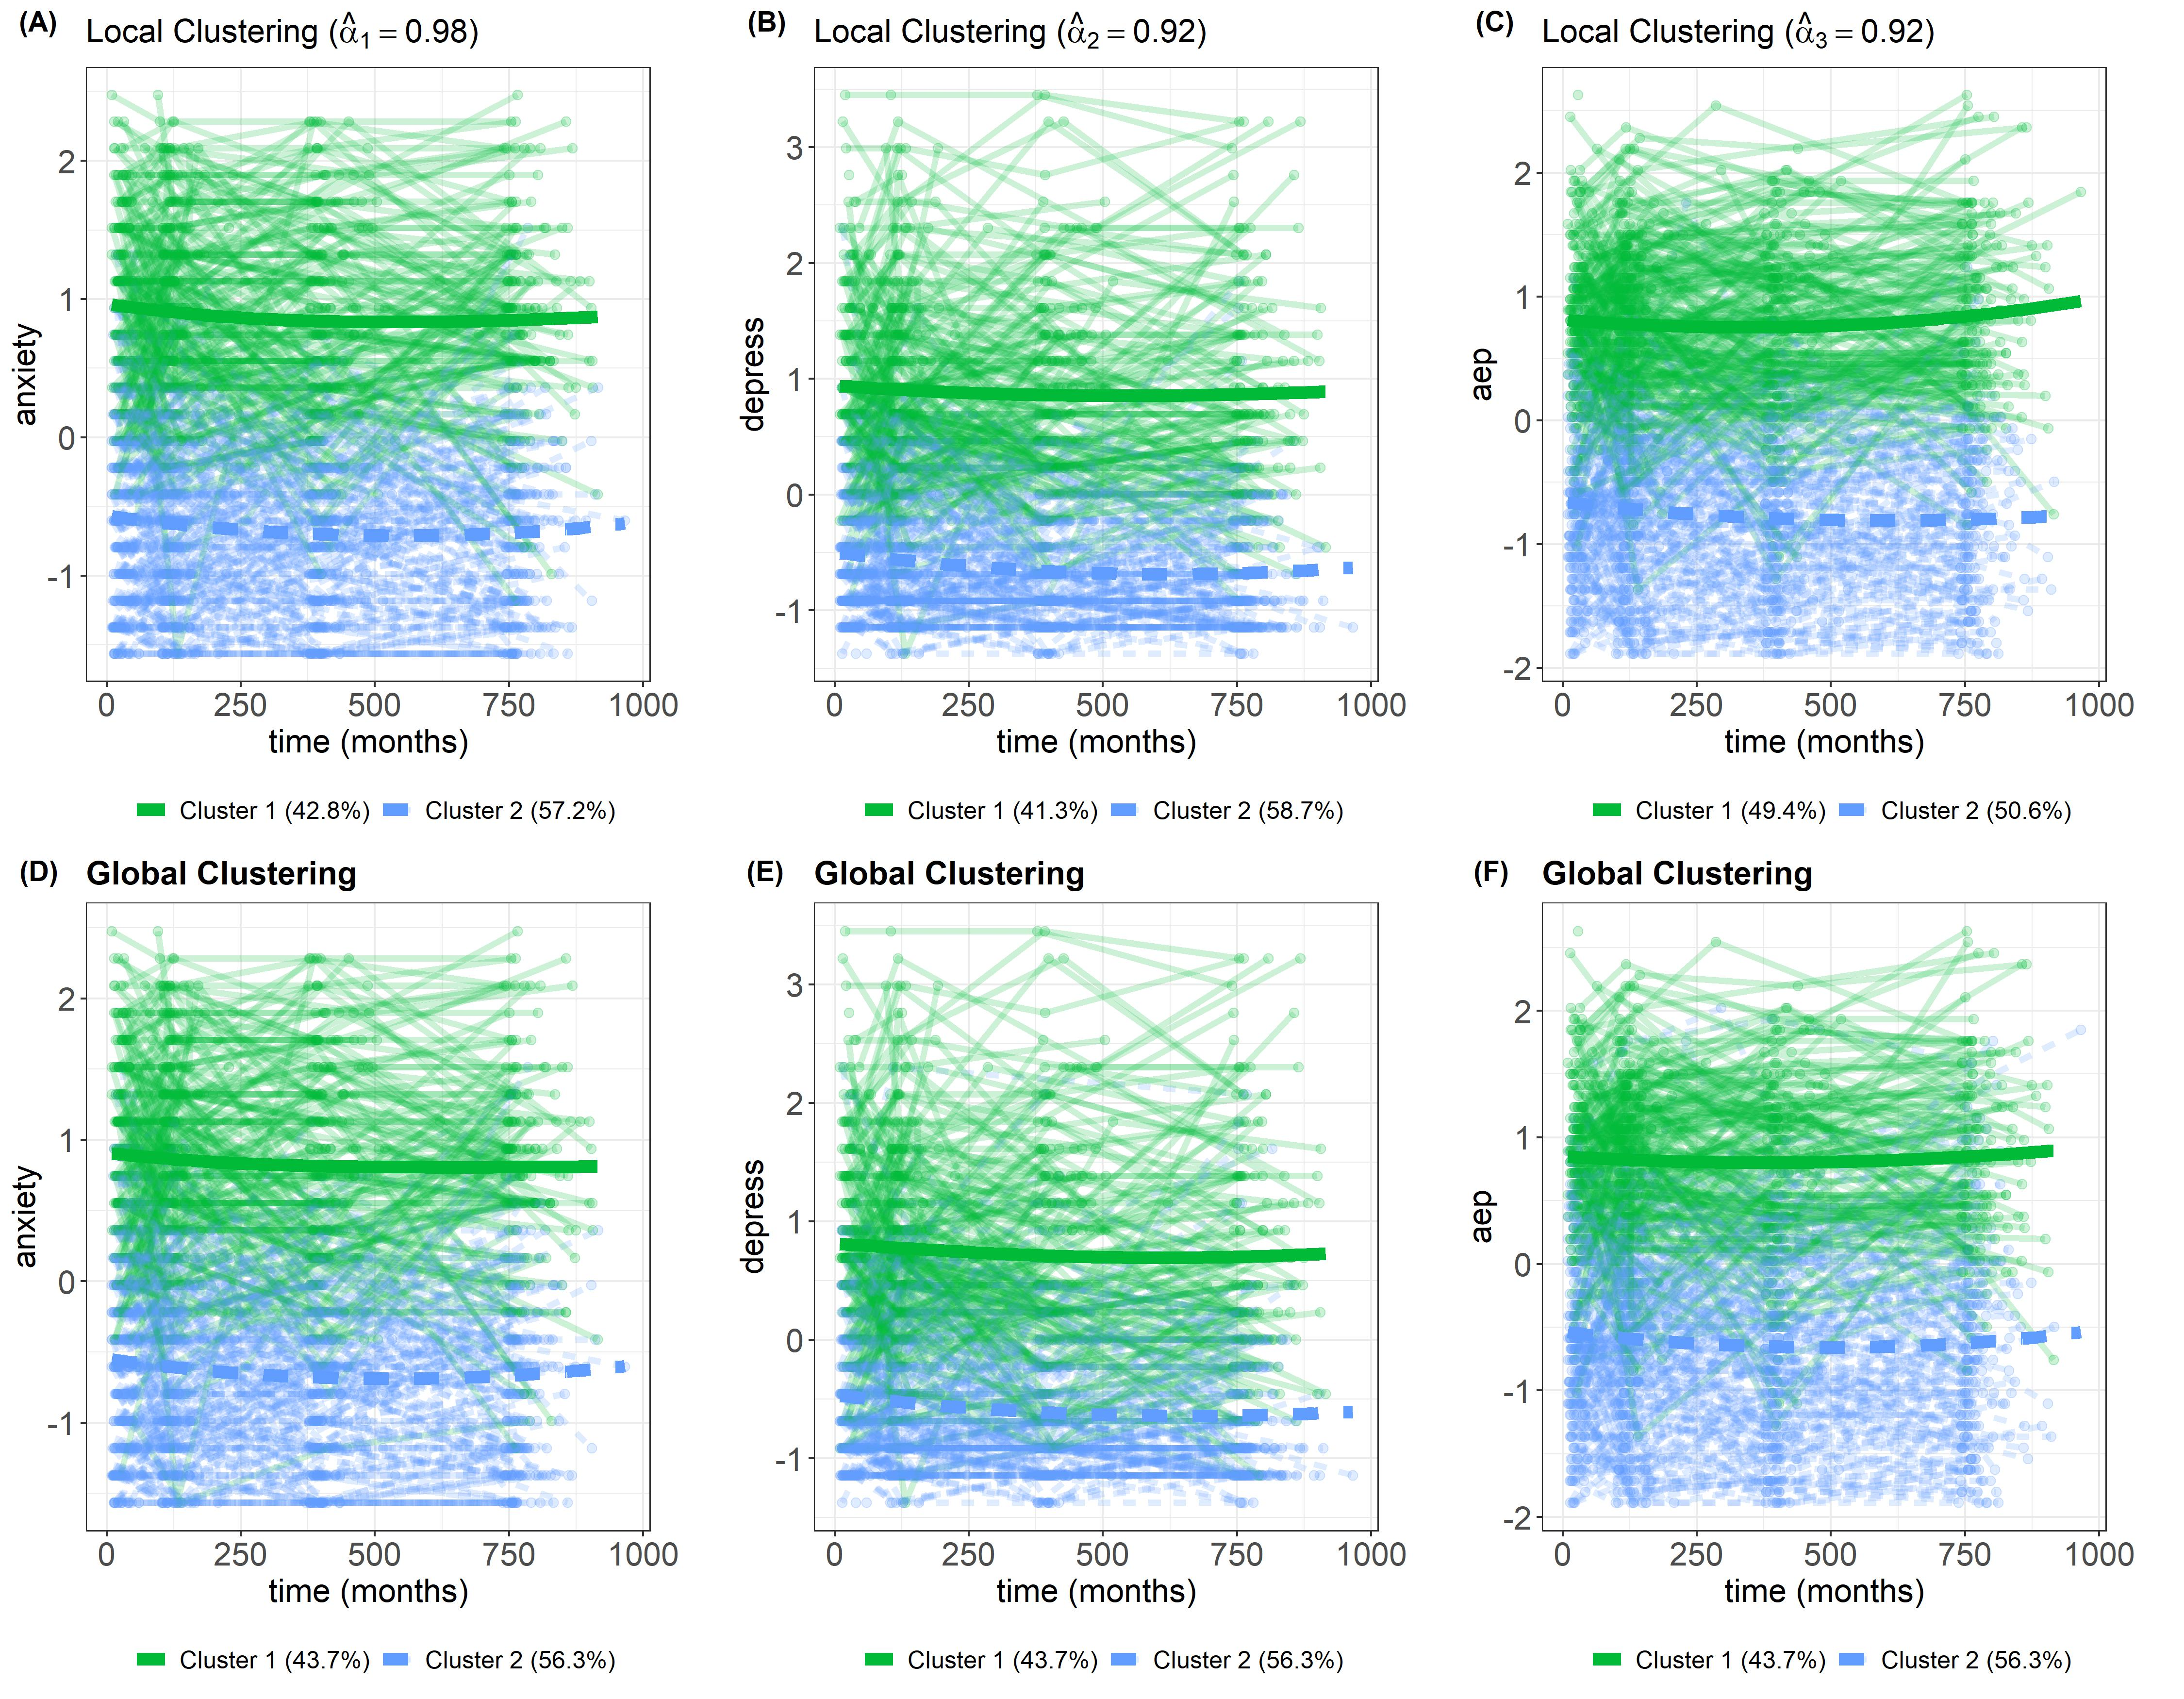
\includegraphics[width=\textwidth,height=10cm]{./Figures/trajplot.JPEG}
\caption{\label{fig:traj_epileptic_qol} Longitudinal trajectories for features by local and global clusterings \textbf{epileptic.qol} data. Locally weighted scatterplot smoothing curves are overlaid on each panel to provide an estimate of the overall trend. (A) Longitudinal trajectories of anxiety plotted by local clustering $\boldsymbol{L}_1$. (B) Longitudinal trajectories of depress plotted by local clustering $\boldsymbol{L}_2$. (C) Longitudinal trajectories of aep plotted by local clustering $\boldsymbol{L}_3$. (D) Longitudinal trajectories of anxiety plotted by global clustering $\boldsymbol{C}$. (E)  Longitudinal trajectories of depress plotted by global clustering $\boldsymbol{C}$. (F)  Longitudinal trajectories of aep plotted by global clustering $\boldsymbol{C}$.}
\end{figure}
\subsubsection{Goodness of Fit}
To assess the model goodness of fit, one can use \textbf{BayesT()} for computing the posterior predictive check. The commands of the two-cluster model for \textbf{epileptic.qol} data are as follows: 
\begin{example}
R> res <- BayesT(fit = fit.BCC2)
R> plot(log(res$T.obs), log(res$T.rep), xlim = c(8.45,8.7), ylim = c(8.45,8.7), cex = 1.5,
+        xlab = "Observed T statistics (in log scale)", 
+        ylab = "Predicted T statistics (in log scale)")
R> abline(0, 1, lwd = 2,col = 2)
\end{example} 
\begin{figure}[h]
\centering
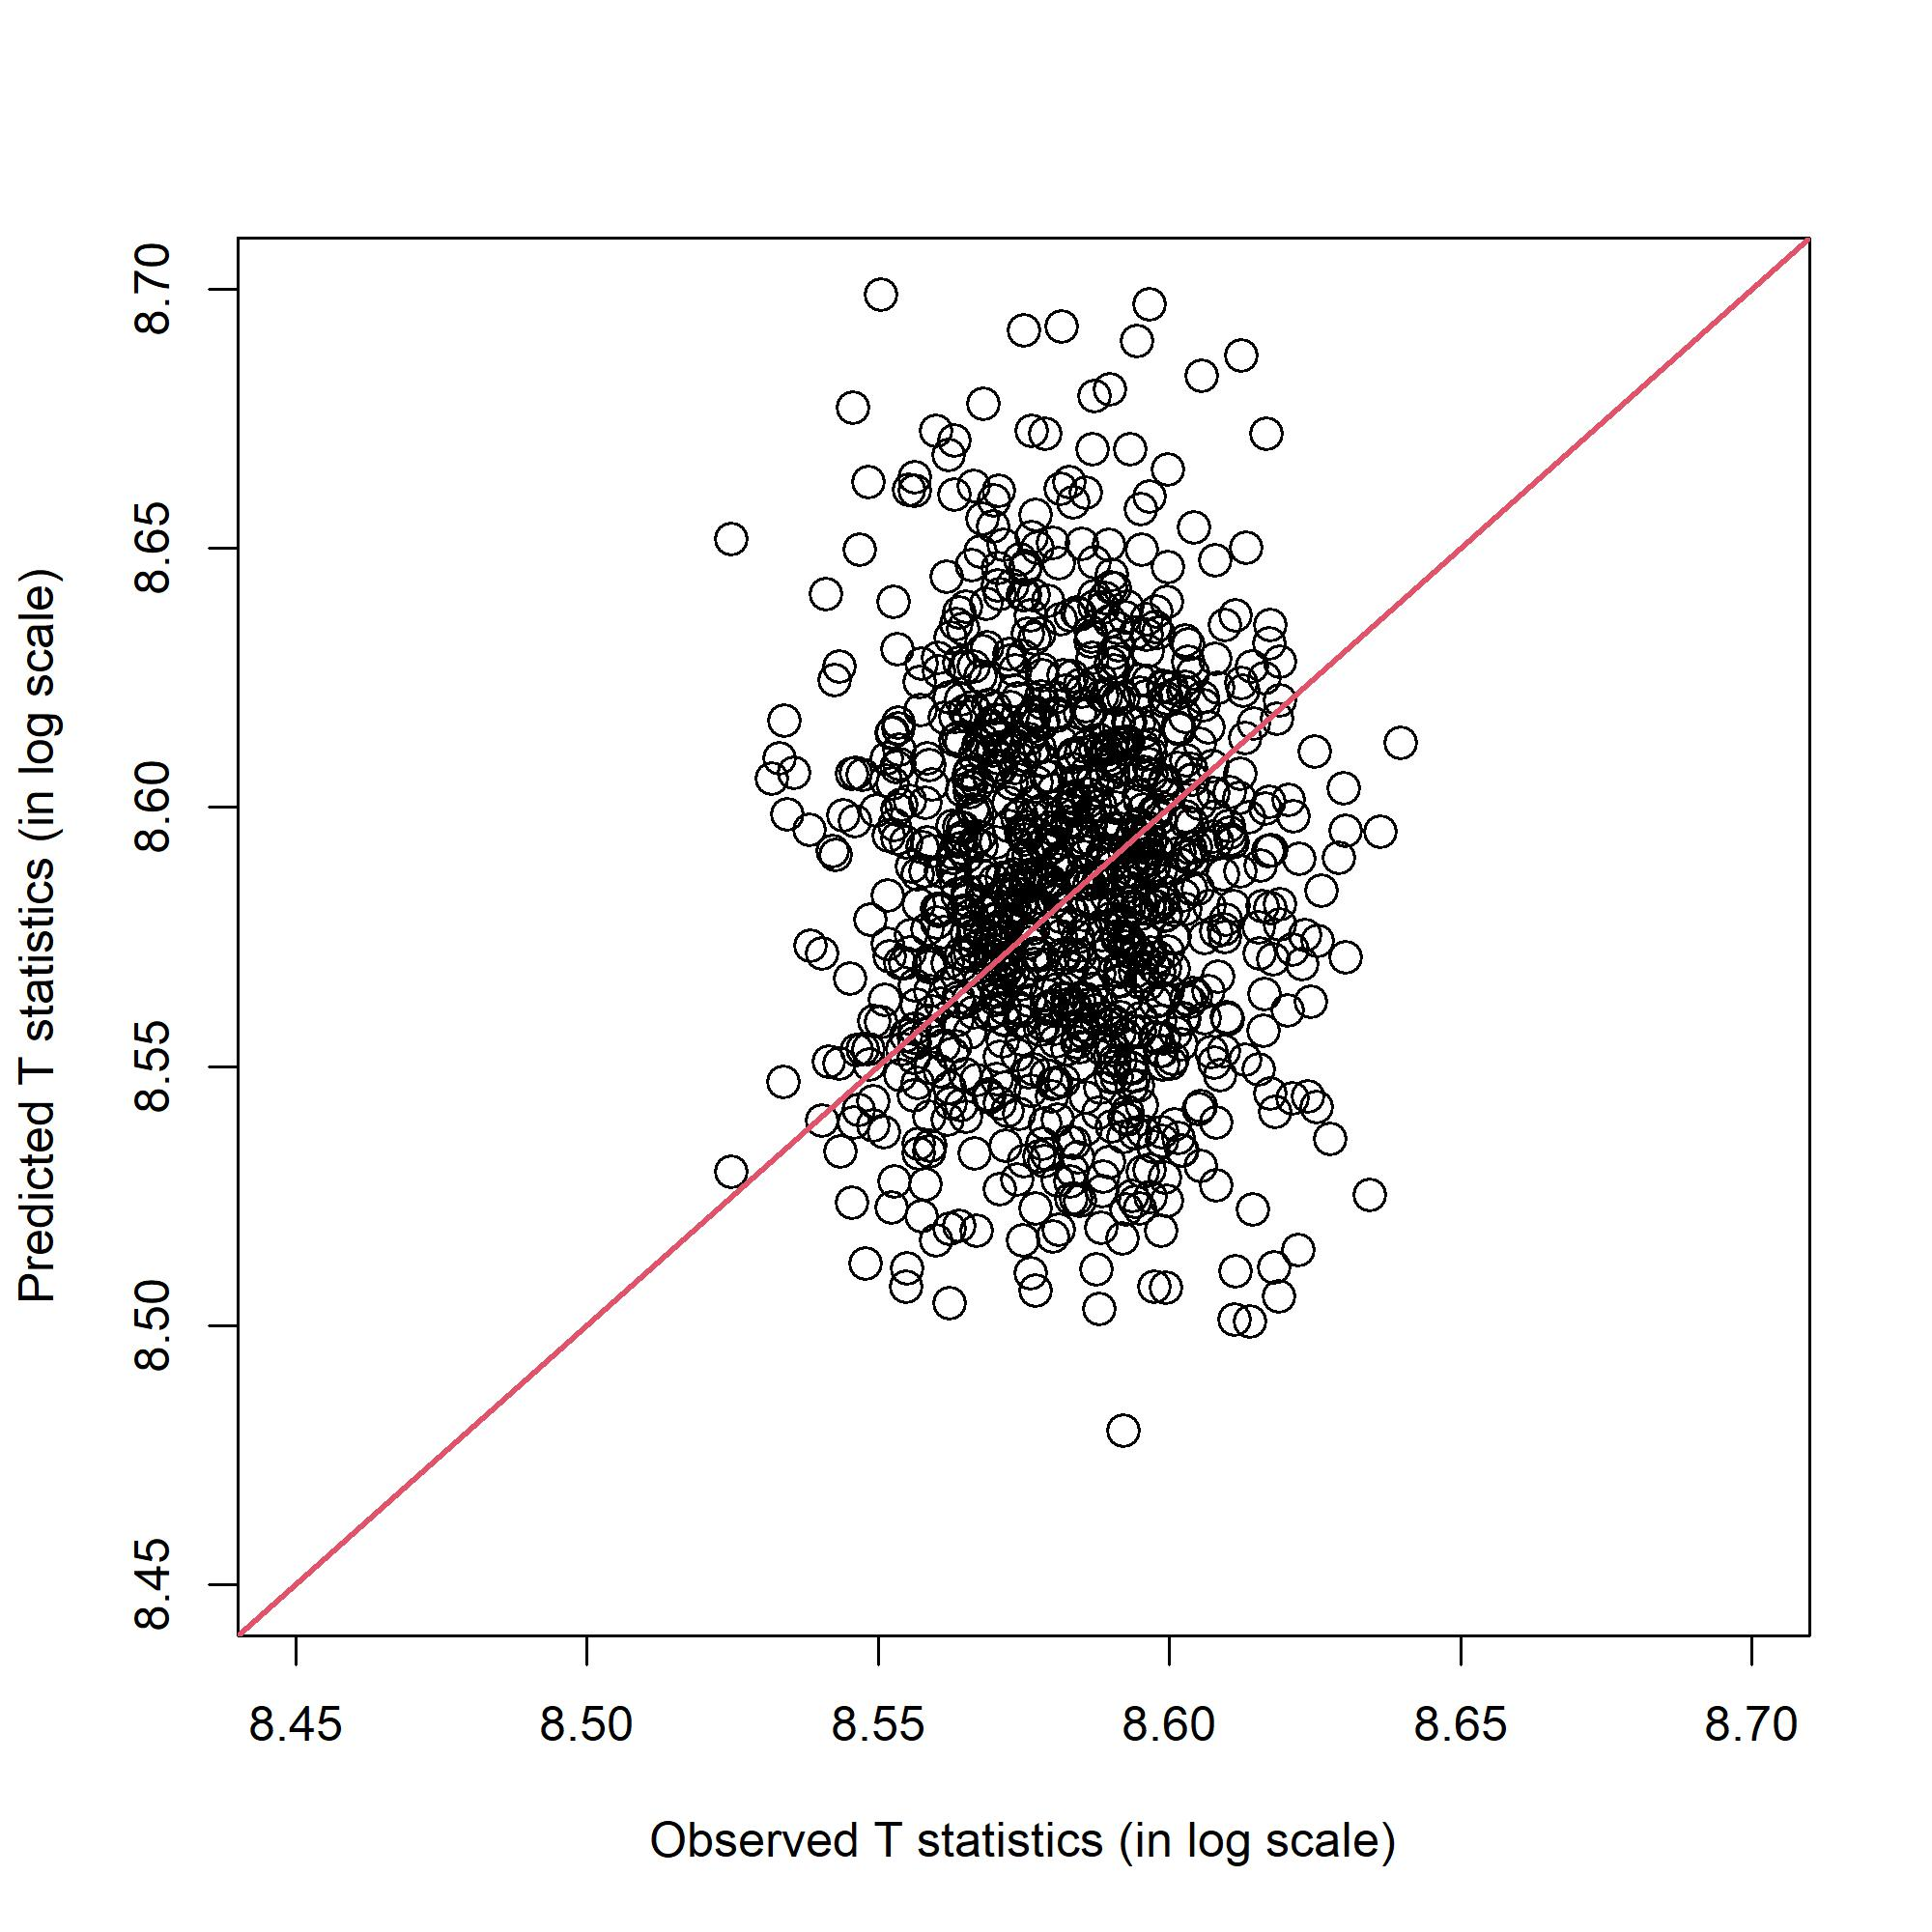
\includegraphics[width=9cm,height=9cm]{./Figures/posterior_check.JPEG}
\caption{\label{fig:posterior_check}  Posterior predictive check: observed $T$ (in log scale) and predicted $T$ (in log scale) statistics.}
\end{figure}
The result is displayed in Figure \ref{fig:posterior_check}. This figure suggested that there was no systematic pattern (e.g., consistent overestimation or underestimation) between the observed $T$ (in log scale) and predicted $T$ (in log scale) statistics, indicating that the model provided a good fit to the data. To further evaluate the goodness of fit using an objective measure, the Bayesian p-value can be calculated, using the following commands,
\begin{example}
R> p.value <- sum(res$T.rep > res$T.obs)/length(res$T.rep)
R> p.value 
\end{example} 
\begin{example}
[1] 0.559
\end{example}
The Bayesian p-value of 0.559 corresponds to the proportion of samples above the diagonal, further suggesting that there is no clear evidence of model misspecification or that the model provides a poor fit to the data. In addition, the output also provided the posterior cluster probability, which is a measure of cluster uncertainty. The following commands generated a boxplot for the posterior cluster probabilities by clusters. 
\begin{example}
R> fit.BCC2$cluster.global <- factor(fit.BCC2$cluster.global,
+        labels = c("Cluster 1", "Cluster 2"))
R> boxplot(fit.BCC2$postprob ~ fit.BCC2$cluster.global, ylim = c(0.5, 1),
+        xlab = "", ylab = "Posterior Cluster Probability")
\end{example} 
The results were displayed in Figure \ref{fig:posterior_prob}. The posterior cluster probabilities for a majority of individuals in both Clusters 1 and 2 were close to 1, except for a few individuals. This suggested that the cluster membership for individuals is robust. 
\begin{figure}[t!]
\centering
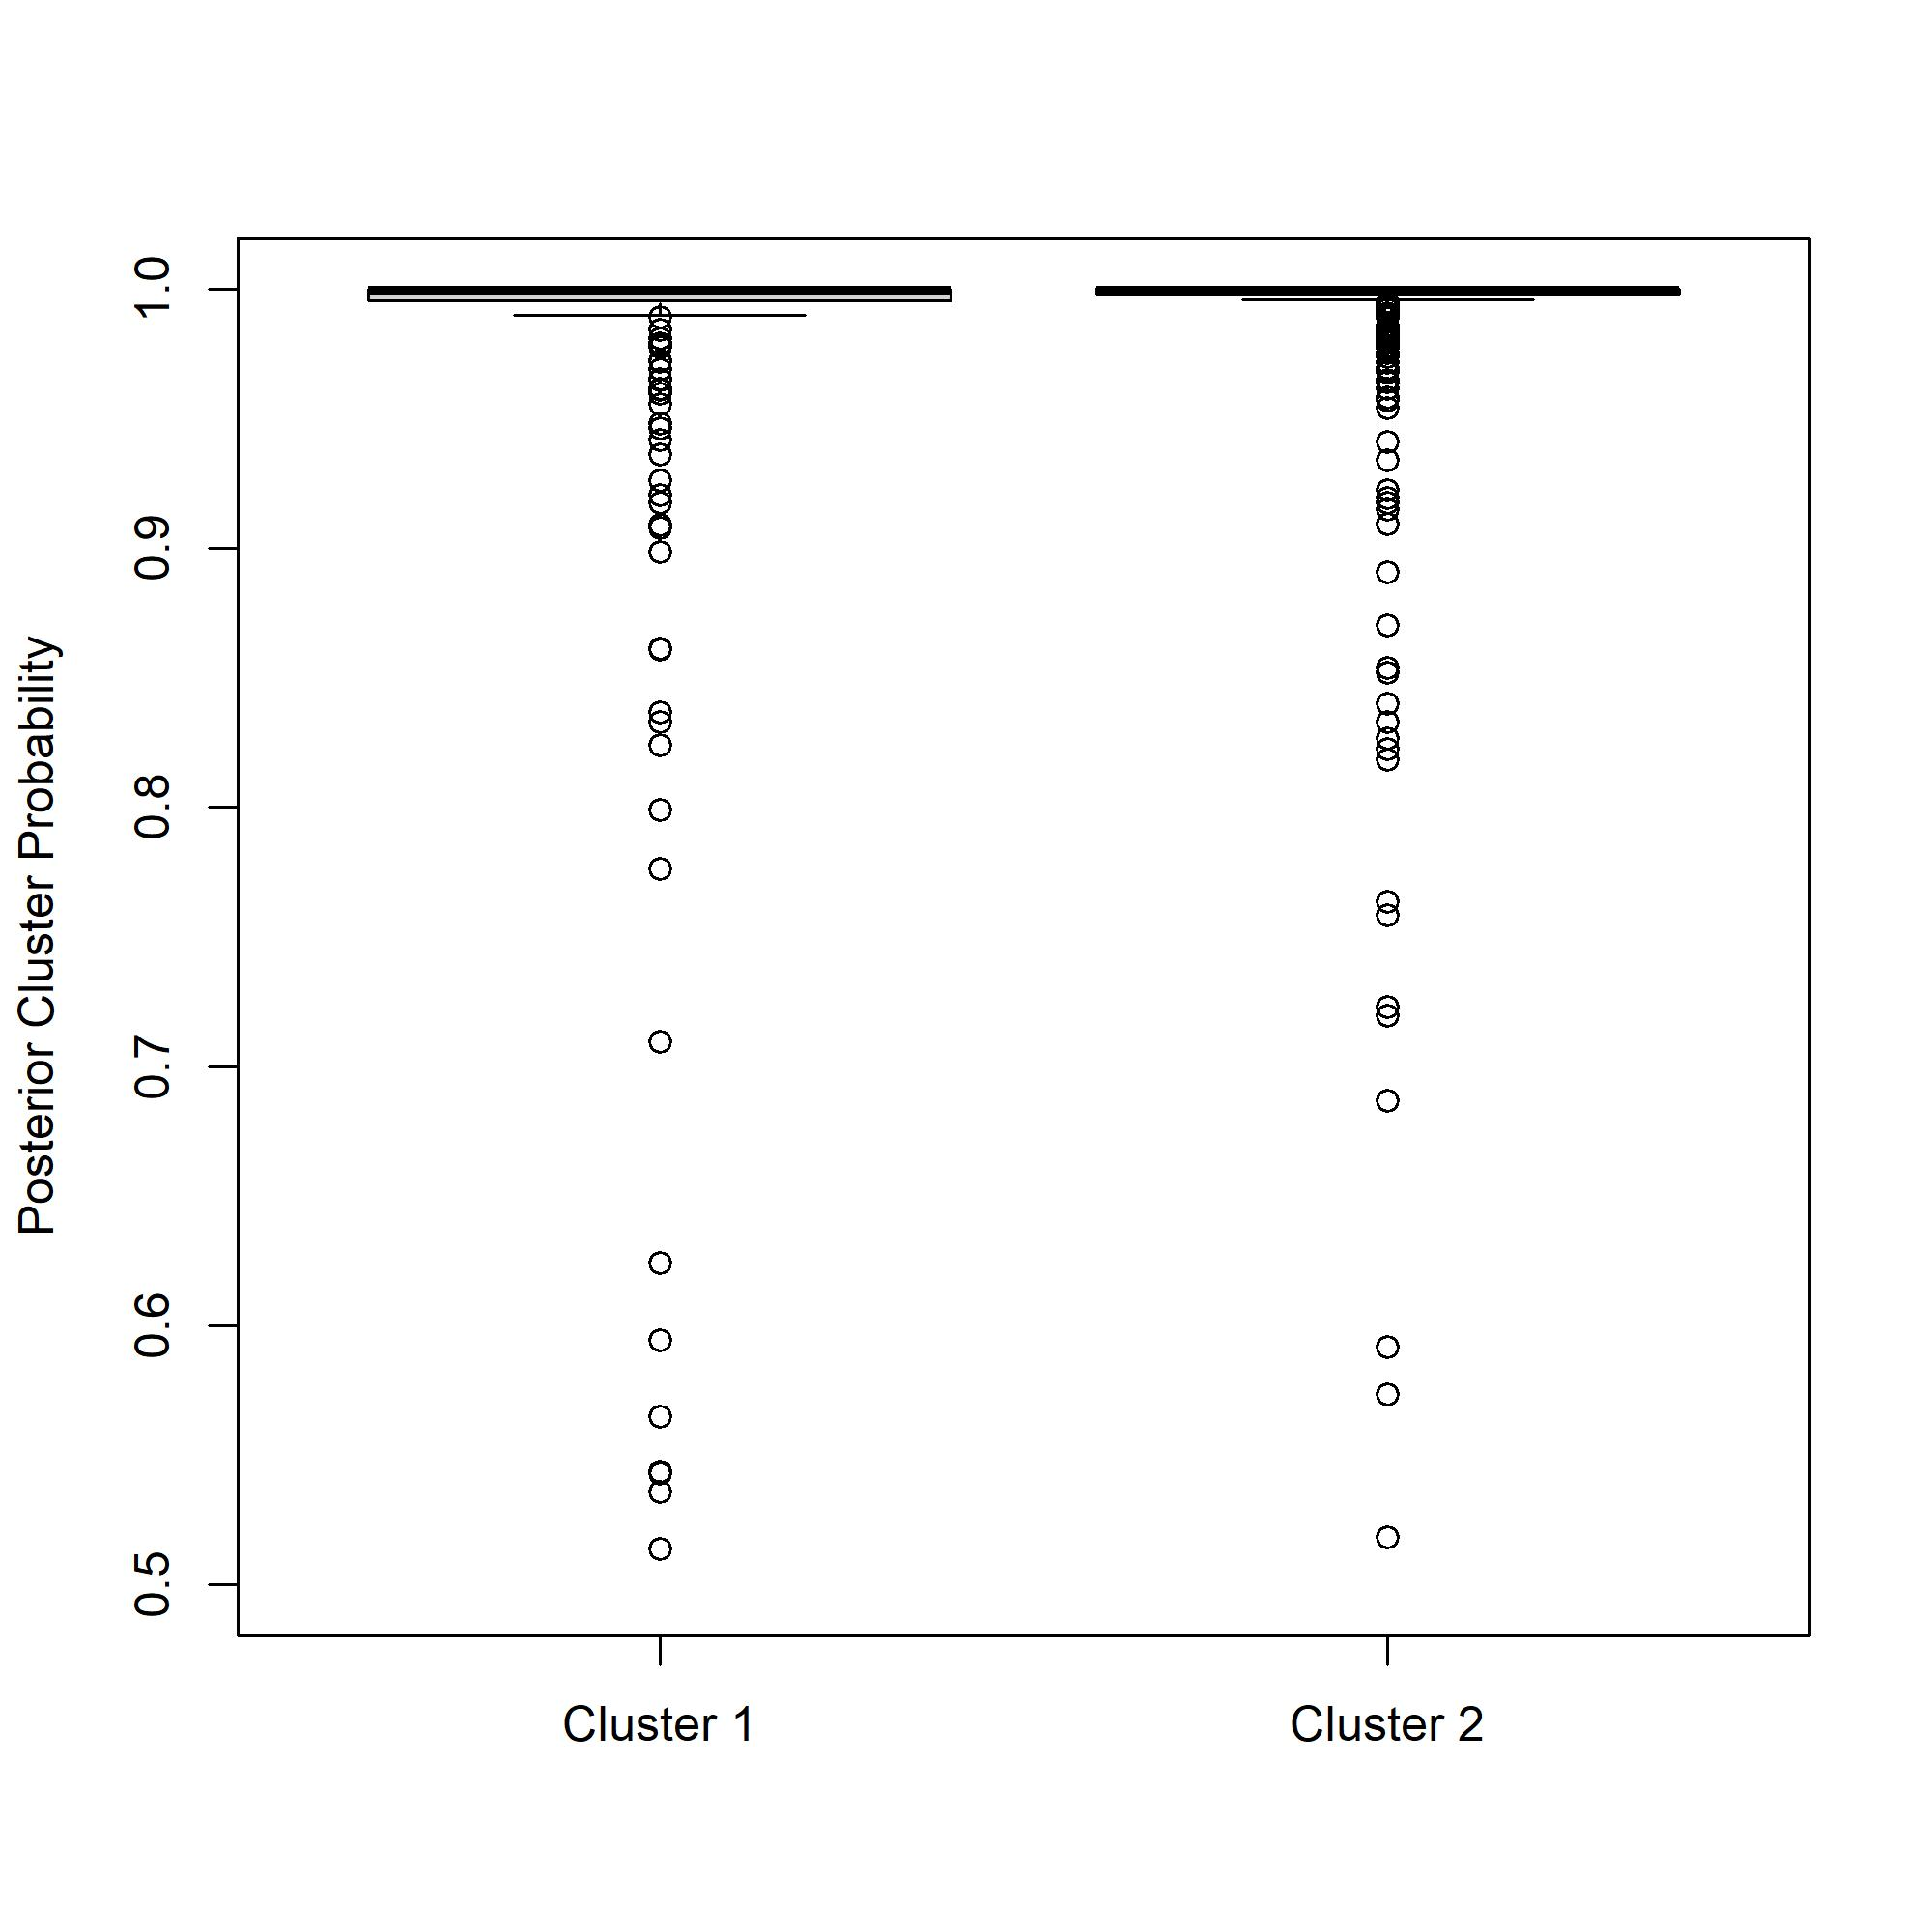
\includegraphics[width=9cm,height=9cm]{./Figures/posterior_prob.JPEG}
\caption{\label{fig:posterior_prob}  Boxplot for the posterior cluster probabilities by clusters.}
\end{figure}
\subsubsection{Using a Different Set of Initial Values for Local and Global Cluster Memberships}
It is a good practice to fit the model with different starting values to ensure the model converges and the clustering results are stable. By default, the initial values of the local cluster membership are randomly generated from 1 to $K$ for each feature, and the global cluster membership is set to be equal to the local cluster membership of the first feature. One can also supply the local cluster membership by fitting the Bayesian mixture model for longitudinal data to each feature through the mixAK package for the given $K$. To do so, the argument \code{ initial.cluster.membership = "mixAK"} can be added to the \code{BCC.multi} function. One can also provide user input initial values for the cluster membership, by using \code{ initial.cluster.membership = "input"}, and then supply the initial values using the \code{ input.initial.local.cluster.membership} and \code{  input.initial.global.cluster.membership} arguments. For example, if the user would like to refit the model using clustering results generated from the previous model  (\code{fit.BCC2}), the following code can be used:  
\begin{example}
> fit.BCC2a <-  BCC.multi (
+        mydat = list(dat$anxiety_scale, dat$depress_scale, dat$aep_scale),
+        dist = c("gaussian"),
+        id = list(dat$id),
+        time = list(dat$time),
+        formula = list(y ~ time + (1|id)),
+        initial.cluster.membership = "input",
+        input.initial.local.cluster.membership = list(fit.BCC2$cluster.local[[1]],
+        fit.BCC2$cluster.local[[2]], fit.BCC2$cluster.local[[3]]),
+        input.initial.global.cluster.membership = fit.BCC2$cluster.global,
+        num.cluster = 2,
+        burn.in = 1000, 
+        thin = 1, 
+        per = 100,  
+        max.iter = 2000)  
\end{example} 
\subsubsection{Comparing Clustering Results to Other Model Specifications}
To evaluate the robustness of the resulting clusters, one can compare the clustering results to more complicated models. We fit a BCC model with a linear form using a random intercept and slope, and a BCC model with a quadratic form using a random intercept and slope. The commands are as follows: 
\begin{example}
R> fit.BCC2b <-  BCC.multi (
+        mydat = list(dat$anxiety_scale, dat$depress_scale, dat$aep_scale),
+        dist = c("gaussian"),
+        id = list(dat$id),
+        time = list(dat$time),
+        formula = list(y ~ time + (1 + time|id)),
+        num.cluster = 2,
+        print.info = "FALSE",
+        burn.in = 1000, 			 
+        thin = 1, 				 
+        per = 100, 				  
+        max.iter = 2000) 
R> fit.BCC2c <-  BCC.multi (
+        mydat = list(dat$anxiety_scale, dat$depress_scale, dat$aep_scale),
+        dist = c("gaussian"),
+        id = list(dat$id),
+        time = list(dat$time),
+        formula = list(y ~ time + time2 + (1 + time|id)),
+        num.cluster = 2,
+        print.info = "FALSE",
+        burn.in = 1000,  
+        thin = 1,  
+        per = 100,  
+        max.iter = 2000) 
> fit.BCC2b$cluster.global <- factor(fit.BCC2b$cluster.global,
+        labels = c("Cluster 1", "Cluster 2"))
> table(fit.BCC2$cluster.global, fit.BCC2b$cluster.global)
\end{example} 
\begin{example}
           Cluster 1 Cluster 2
  Cluster 1       223        13
  Cluster 2         1       303
\end{example}
The agreement between the first model (linear model with a random intercept) and the second model (linear model
with a random intercept and random slope) was $(223 + 303)/540 = 97\%$. 
\begin{example}
R> fit.BCC2c$cluster.global <- factor(fit.BCC2c$cluster.global,
+        labels = c("Cluster 1", "Cluster 2"))
R> table(fit.BCC2$cluster.global, fit.BCC2c$cluster.global)
\end{example} 
\begin{example}
            Cluster 1 Cluster 2
  Cluster 1       227       9
  Cluster 2         2       302
\end{example}
The agreement between the first model (linear model with a random intercept) and the second model (quadratic model with a random intercept and random slope) was $(226 + 301)/540 = 98\%$. This suggested that fitting a more complicated model does not substantially change the individual cluster membership, and further attests that the estimated cluster membership was robust to different model specifications. 
\subsection{Example 2: Mayo Clinic Primary Biliary Cholangitis Data}
The second dataset was from a randomized placebo-controlled trial of the drug D-penicillamine for Primary Biliary Cholangitis conducted between 1974 and 1984 at the Mayo Clinic Primary Biliary Cholangitis (PBC). The dataset used here contains multiple laboratory results collected longitudinally on 312 randomized PBC patients. Example features (variables) include serum bilirubin (mg/dl), serum albumin (mg/dl), platelet count, serum glutamic-oxaloacetic transaminase and the presence of blood vessel malformations in the skin. The dataset was analyzed previously by \citet{Komarek2013} using the \pkg{mixAK} package. The analysis goal was to identify subgroups of patients with similar profiles based on multiple features which may serve as critical information regarding patients’ prognostics.
To illustrate the clustering process of mixed-type longitudinal features, we followed \citet{Komarek2013} analysis and chose three features of interest, namely the lbili (log of serum bilirubin), platelet count, and spiders (presence of blood vessel malformations in the skin). Also, following \citet{Komarek2013}, we included $N = 260$ individuals known to be alive at 910 days of follow-up, and only the longitudinal measurements up to this point were considered (known as the \textbf{PBC910} data). The median (min, max) number of observations for these markers was 4 (1, 5). Given a small number of observations available for each individual, we considered a model with only a random intercept, i.e., using the following specification:
\begin{example}
     		formula = list(y ~ time + (1|id))
\end{example} 
For a complete analysis, one can follow the steps outlined in Example 1 to determine the number of clusters and to evaluate the model performance using several different approaches (e.g., posterior predictive check). Here, as an illustration, and for the purpose of comparison, we only fitted a model with two clusters (i.e., $K=2$) as in \citet{Komarek2013}. 
The data is available through the \pkg{mixAK} package. The following commands prepared the dataset for analysis.
\begin{example}
R> library("mixAK")
R> data(PBC910)
\end{example} 
Using the argument \code{dist = c("gaussian","poisson","binomial")} to specify the distributions for the three features, the following commands performed a BCC model with $K=2$.
\begin{example}
R > fit.BCC2 <- BCC.multi(
+        mydat = list(PBC910$lbili, PBC910$platelet, PBC910$spiders),
+        dist = c("gaussian", "poisson", "binomial"),
+        id = list(PBC910$id),
+        time = list(PBC910$month),
+        formula = list(y ~ time + (1|id)),
+        num.cluster = 2,
+        burn.in = 10000,   
+        thin = 10,     
+        per = 1000,       
+        max.iter = 20000)
\end{example} 
The following commands generated the longitudinal profile plots for the three features (lbili, platelet, spiders). 
\begin{example}
R> gp1 <- trajplot(fit = fit.BCC2, feature.ind = 1, 
+        which.cluster = "local.cluster",
+        title = bquote(paste("Local Clustering (",
+        hat(alpha)[1] ==.(round(fit.BCC2$alpha[1],2)),")")),
+        xlab = "months", ylab = "lbili", color = c("#00BA38", "#619CFF"))
R> gp2 <- trajplot(fit = fit.BCC2, feature.ind = 2, 
+        which.cluster = "local.cluster",
+        title = bquote(paste("Local Clustering (",
+        hat(alpha)[2] ==.(round(fit.BCC2$alpha[2],2)),")")),
+        xlab = "months", ylab = "platelet", color = c("#00BA38", "#619CFF"))
R> gp3 <- trajplot(fit = fit.BCC2, feature.ind = 3, 
+        which.cluster = "local.cluster",
+        title = bquote(paste("Local Clustering (",
+        hat(alpha)[3] ==.(round(fit.BCC2$alpha[3],2)),")")),
+        xlab = "months", ylab = "spiders", color = c("#00BA38", "#619CFF"))
R> gp4 <- trajplot(fit = fit.BCC2, feature.ind = 1, 
+        which.cluster = "global.cluster",
+        title = "Global Clustering",
+        xlab = "months", ylab = "lbili", color = c("#00BA38", "#619CFF"))
R> gp5 <- trajplot(fit = fit.BCC2, feature.ind = 2, 
+        which.cluster = "global.cluster",
+        title = "Global Clustering",
+        xlab = "months", ylab = "platelet", color = c("#00BA38", "#619CFF"))
R> gp6 <- trajplot(fit = fit.BCC2, feature.ind = 3, 
+        which.cluster = "global.cluster",
+        title = "Global Clustering",
+        xlab = "months", ylab = "spiders", color = c("#00BA38", "#619CFF"))
\end{example} 
\begin{figure}[h]
\centering
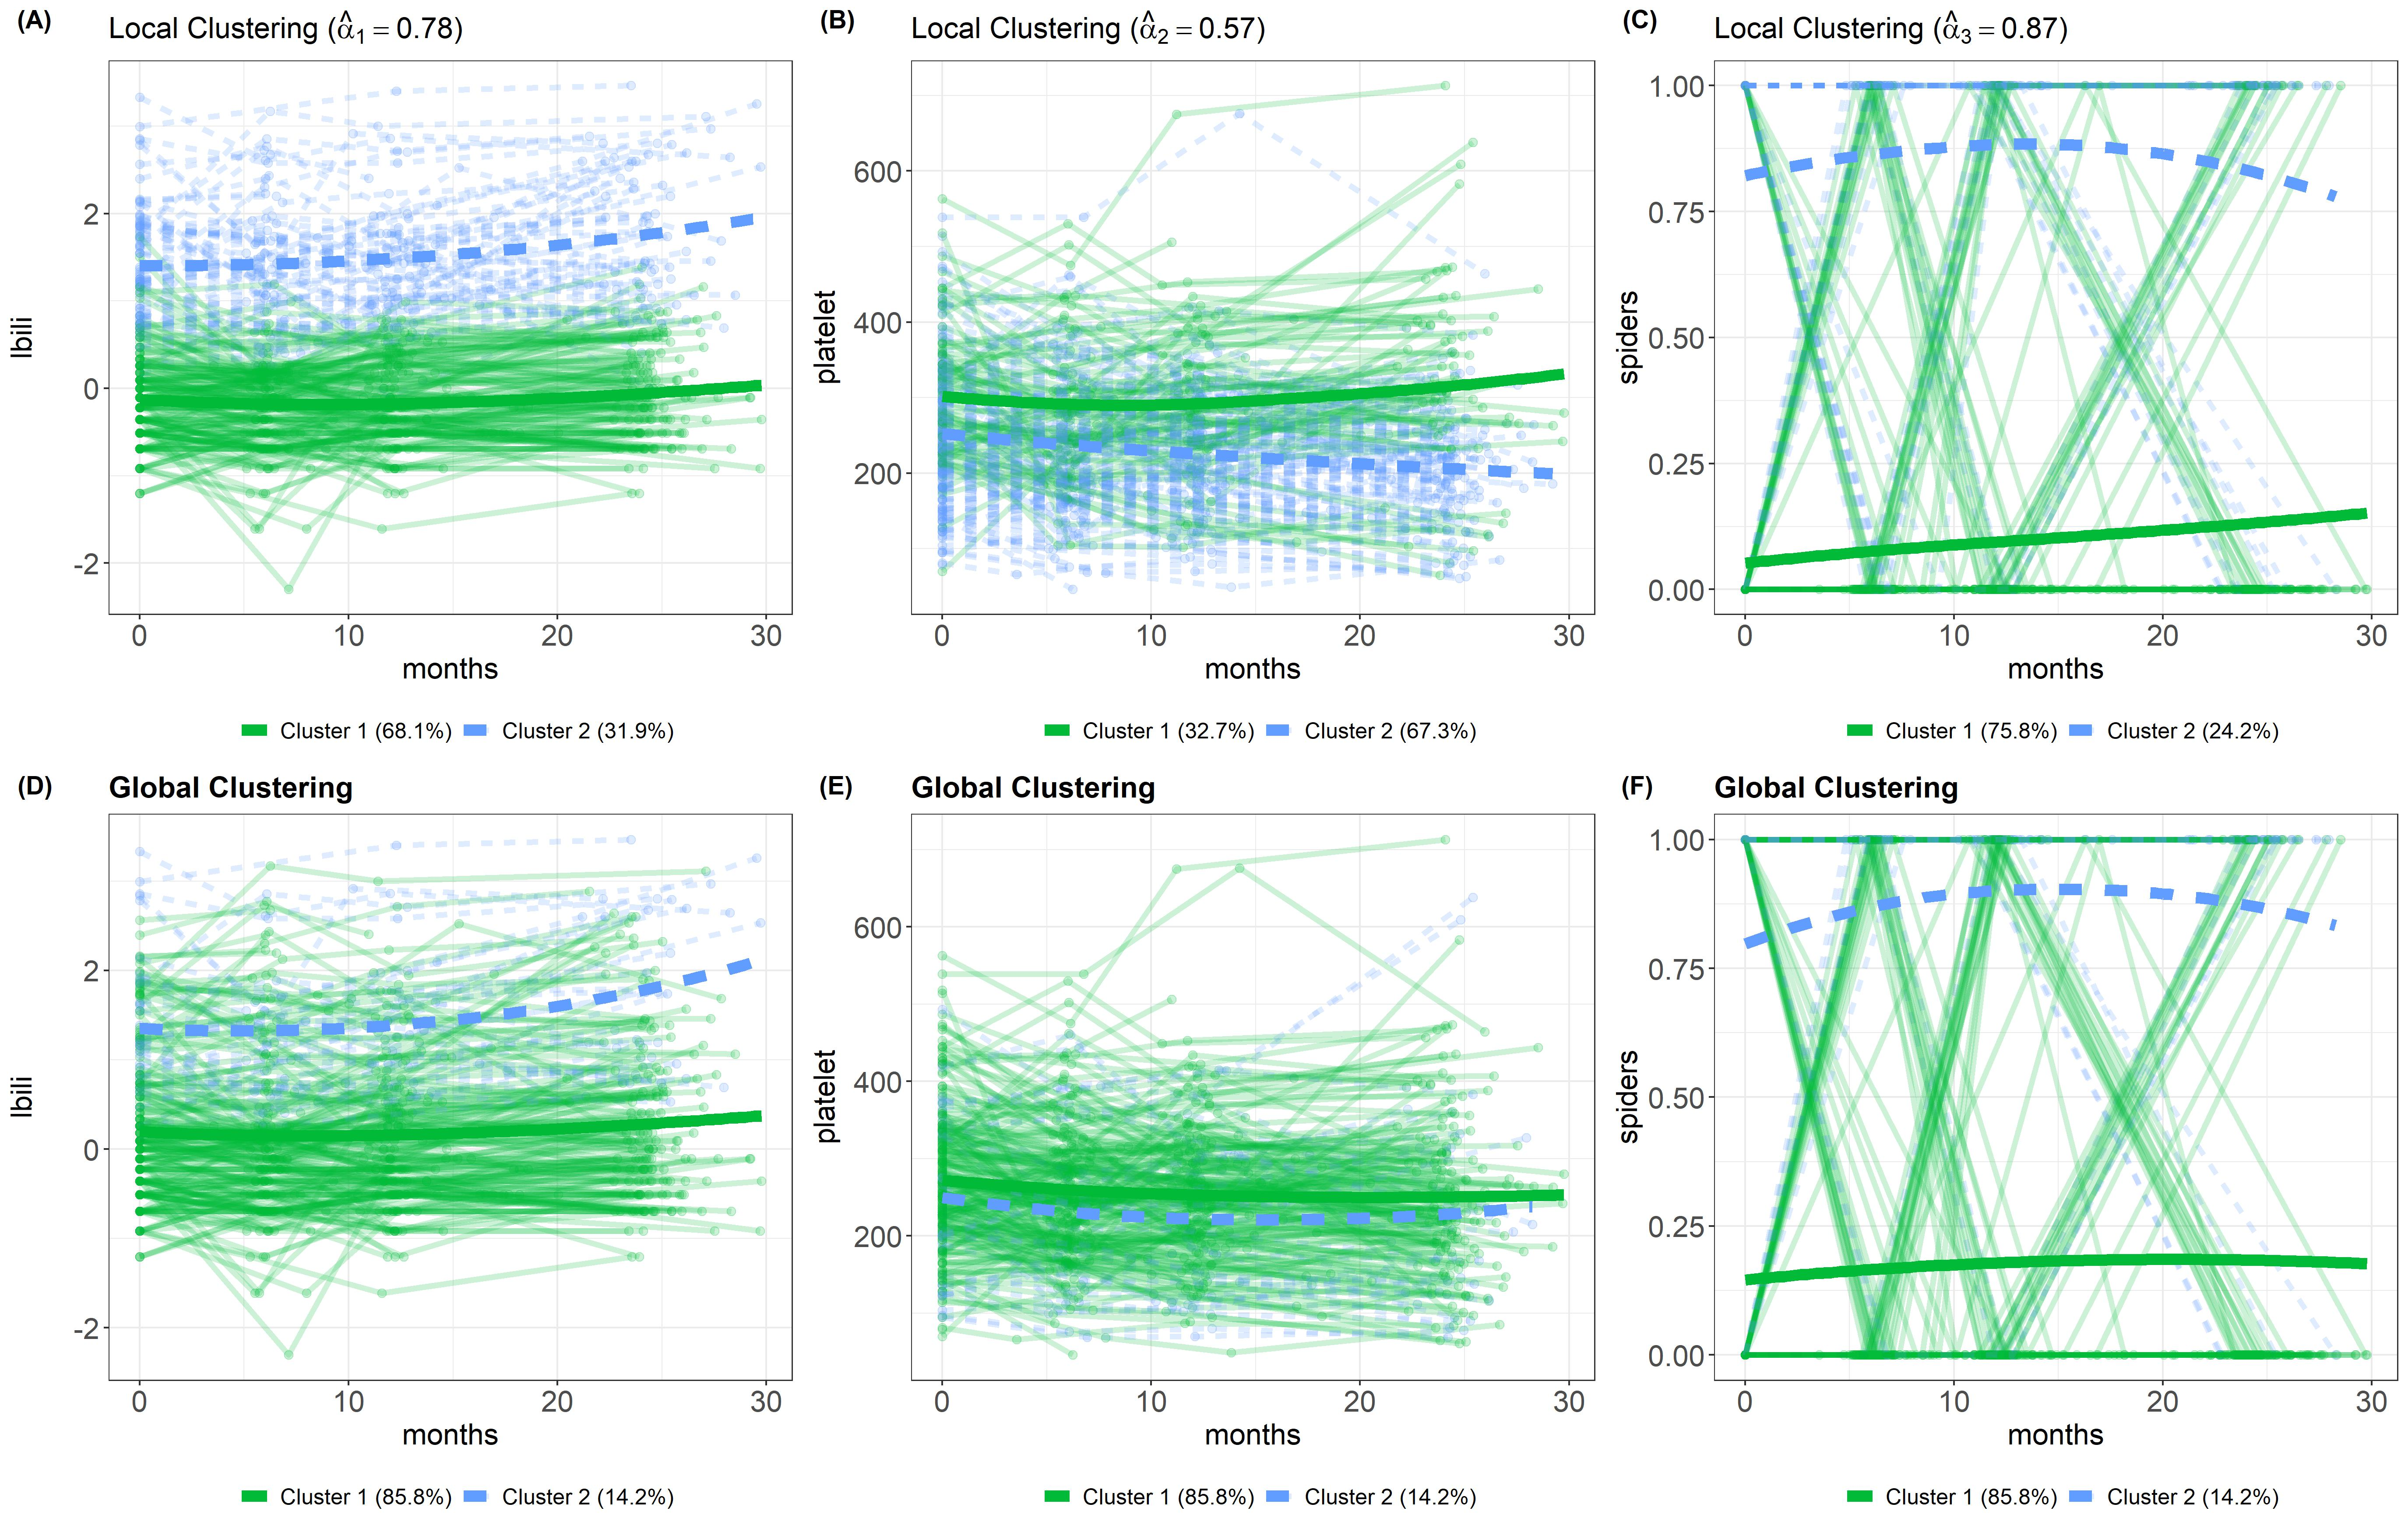
\includegraphics[width=\textwidth,height=10cm]{./Figures/trajplot_PBC910.JPEG}
\caption{\label{fig:traj} Longitudinal trajectories for features by local and global clusterings for \textbf{PBC910} data. Locally weighted scatterplot smoothing curves are overlaid on each panel to provide an estimate of the overall trend.  (A) Longitudinal trajectories of lbili plotted by local clustering $\boldsymbol{L}_1$. (B) Longitudinal trajectories of platelet plotted by local clustering $\boldsymbol{L}_2$. (C) Longitudinal trajectories of spiders plotted by local clustering $\boldsymbol{L}_3$. (D) Longitudinal trajectories of lbili plotted by global clustering $\boldsymbol{C}$. (E)  Longitudinal trajectories of platelet plotted by global clustering $\boldsymbol{C}$. (F)  Longitudinal trajectories of spiders plotted by global clustering $\boldsymbol{C}$.}
\end{figure}
To compare the results with an existing model, we fit a Bayesian mixture model using the \pkg{mixAK} package using the following commands (see \citep{Komarek2014} for details of using this package): 
\begin{example}
R> mod <- GLMM_MCMC(y = PBC910[, c("lbili", "platelet", "spiders")],
+        dist = c("gaussian", "poisson(log)", "binomial(logit)"),
+        id = PBC910[, "id"], 
+        x = list(lbili = "empty", platelet = "empty", spiders = PBC910[, "month"]), 
+        z = list(lbili = PBC910[, "month"], platelet = PBC910[, "month"], spiders = "empty"),
+        random.intercept = rep(TRUE, 3), prior.b = list(Kmax = 2),
+        nMCMC = c(burn = 100, keep = 1000, thin = 10, info = 100),
+        parallel = FALSE)
R> mod <- NMixRelabel(mod, type = "stephens", keep.comp.prob = TRUE)
R> cluster.mixAK <- apply(mod[[1]]$poster.comp.prob, 1, which.max)
R> table(mixAK = cluster.mixAK, BCClong = fit.BCC2$cluster.global)
\end{example} 
\begin{example}
     BCClong
mixAK   1   2
    1 158   3
    2  65  34
\end{example}
The agreement between the two models for the \textbf{PBC910} data was (158 + 34)/260 = 74\%.
\section{Summary and discussion} \label{sec:summary}
In this paper, we described a BCC model for clustering longitudinal data with multiple features. Using two real-life and open-access data, we provided step-by-step guidance on using the \pkg{BCClong} package and interpreting the results. The results also demonstrated that the \pkg{BCClong} package is a useful tool for clustering longitudinal data and it enhanced our understanding of the heterogeneity underlying each feature and across features. Of note, the reason we require the user to create three separate lists of data vectors (instead of a data frame) when using BCC.multi(), in specifying the arguments mydat, id, and time is to allow more flexibility in modeling longitudinal features with distinct structures. This is particularly useful when these features are collected from multiple data sources (with different study designs), and therefore the time scale and data collection frequency could differ between features. Additional details regarding the functions and their arguments can be found in the package vignettes.
The BCC model implemented using the \pkg{BCClong} package yields both feature-specific (local) clusterings and consensus (global) clustering. In practice, global clustering is often of greater interest, as it encompasses information from all features. It can be used to associate with exposures and predict long-term outcomes. Conceptually, feature-specific clustering can be viewed as clustering based on a single feature alone, whereas global clustering can be viewed as a weighted average clustering across all features, with weights being the adherence parameters. In order to capture the complexity of the underlying population heterogeneity, it is of great importance to consider multiple features of interest simultaneously, as we often do for cross-sectional data. 
Several directions can be considered in future studies. For example, incorporating variable selection (e.g., spike-and-slab and shrinkage) priors \citep{Lu2021b, Lu2021} for fixed and random effects will enhance the flexibility of the package and allow it to be applied to high-dimensional settings. In addition, determining the number of clusters can be achieved by using a Dirichlet process mixture model \citep{Escobar1994, Lu2023a, Lu2024}. The package does not support predicting the cluster membership of a new individual or future trajectories for a given individual. These functions will be considered in future versions of the package. Finally, the current version of the \pkg{BCClong} package relies on a standard MCMC algorithm to estimate the model, which is generally slow and requires particular care for the user to check convergence. While the computational time is reasonable for our current applications, to scale up the model to a large dataset, other computational algorithms such as distributed stochastic gradient MCMC \citep{Ahn2014} and variational inference \citep{Blei2017} can be considered in future studies.
\section*{Computational details}
Most of the functions in the \pkg{BCClong} package are written in C++. The output shown in this article was obtained using R version 4.2.1 (June, 2022), \pkg{BCClong} 1.0.3, and the following contributed packages which are the dependencies or imports of the \pkg{BCClong} package: cluster (2.1.4) \citep{Maechler2022}, coda (0.19-4) \citep{Martyn2006}, ggplot2 (3.4.0) \citep{Wickham2016}, label.switching (1.8) \citep{Papastamoulis2016}, LaplacesDemon (16.1.6) \citep{Hall2022}, lme4 (1.1-31) \citep{Bates2015}, MASS (7.3-58.1) \citep{Ripley2013}, mclust (6.0.0) \citep{Fraley2006}, MCMCpack (1.6-3) \citep{Martin2011}, mixAK (5.5) \citep{Komarek2014}, mvtnorm (1.1-3) \citep{Genz2021}, nnet (7.3-18) \citep{Ripley2016}, Rcpp (1.0.9) \citep{Eddelbuettel2011}, Rmpfr (0.8-9) \citep{Maechler2022a}, truncdist (1.0-2) \citep{Novomestky2016}. R itself and all packages used are available from the Comprehensive R Archive Network (CRAN) at \url{https://CRAN.R-project.org/}.
\section*{Acknowledgments}
ZT is supported by a Dean’s Doctoral Award from Queen’s University. ZL is supported by a Discovery Grant funded by the Natural Sciences and Engineering Research Council of Canada.
\bibliography{BCClong}
\address{Zhiwen Tan\\
  Department of Public Health Sciences\\
  Queen's University}
\address{Chang Shen\\
  Department of Electrical and Computer Engineering\\
  Queen's University}
\address{Zihang Lu\\
  Department of Public Health Sciences\\
  \emph{and} Department of Mathematics and Statistics\\
  Queen's University\\
  \email{zihang.lu@queensu.ca}}
